\chapter{Applications}\label{ch:appls}
In this chapter, we now apply the theoretical developments of \Cref{ch:linear_theory} and the mixture model algorithm described in \Cref{ch:gmm} to two different applications, using models constructed from observed data.
We do not investigate any of these four applications in detail; rather, the aim is to demonstrate the applicability of the theory to a range of examples.


The first example is a stochastic model constructed from altimetry-derived velocity data of the surface of the Gulf Stream, a climatically important part of the North Atlantic ocean.
This model is 2-dimensional, and in the spirit of stochastic sensitivity we constrcut a deterministic model and use the solutions of it t o apprximate a more ``correct'' stochastic counterpart.


\section{The Hellinger distance}
To quantitatively evaluate the performance of the Gaussian approximation and our mixture model, we will use the Hellinger distance to measure the distance between probability distributions.
The Hellinger distance is an example of an \(f\)-divergence, a broader class of measures between two probability distributions.
For two continuous probability distributions in \(\R^n\) with PDFs \(p\) and \(q\), the Hellinger distance between the two distributions is given by
\begin{equation}\label{eqn:hell_dist}
	D_H\!\left(p, q\right) = \sqrt{\frac12 \int_{\R^n}{\left(\sqrt{p(x)} - \sqrt{q(x)}\right)^2\dif x}} = \sqrt{1 - \int_{\R^n}{\sqrt{p(x)q(x)}\dif x}}.
\end{equation}
We previously discussed the Kullback-Leibler divergence---this measure was used by \citet{Sanz-AlonsoStuart_2017_GaussianApproximationsSmall} to quantify the performance of Gaussian approximations to SDE solutions and is another example of an \(f\)-divergence---but choose to use the Hellinger distance here.
There are several attractive properties of the Hellinger distance that lead to us preferring it: the Hellinger distance is both symmetric and defines a metric on the space of probability measures, unlike the KL-divergence.
Moreover, the Hellinger distance always takes values in the interval \([0,1]\), whereas the KL-divergence can become infinite.

Since the models we will be working with cannot be solved exactly, we will use stochastic samples as our ground `truth`, obtained either via a numerical solver (in the case of SDEs) or Gillespie simulation (in the case of population processes).
That is, without access to the true solutions to our model, we instead take a large number of stochastic samples and compare our approximations to those.
This fits in with the philosophy of our aims; the stochastic sampling approach is the standard in practice, and we seek approximations that give the same conclusions without the computational expense.

However, working with stochastic samples from a continuous density presents a complication in using \cref{eqn:hell_dist} to compute the Hellinger distance: the calculation requires evaluation of the probability density function from which these realisations were sampled.
This would require a choice for how to evaluate the density function and then compute the integral in \cref{eqn:hell_dist}; one option is to construct a kernel density estimator from the samples, where a certain known distribution (usually a Gaussian) is placed at each point and then combined into a mixture density.
To avoid the need, we will instead use an \emph{empirical} estimator for the Hellinger distance that approximates \cref{eqn:hell_dist} without having to evaluate either probability density function.
Although we will be comparing the numerical realisations to analytically available probability density functions (from either a single Gaussian approximation of the mixture model algorithm---the availability of the PDFs is another advantage of these methods over Monte-Carlo simulation), we will generate samples from both distributions to use a purely empirical estimator.

Specifically, we will employ the empirical estimator proposed by \citet{DingMullhaupt_2023_EmpiricalSquaredHellinger}, which extends a similar estimator for the KL-divergence by \citet{Perez-Cruz_2008_KullbackLeiblerDivergenceEstimation} to a broader class of divergences, including the Hellinger distance.
Let \(\set{\hat{x}_1, \dotsc, \hat{x}_N}\) and \(\set{\hat{y}_1, \dotsc, \hat{y}_N}\) denote the two sets of realisations from the distributions \(P\) and \(Q\) respectively.
The estimator is derived from the empirical cumulative density functions of each set of samples, and is first computed as
\begin{equation}\label{eqn:hell_emp_Ha}
	\hat{H}_a^2\!\left(P,Q\right) = 1 - \frac{\sqrt{N - 1}\left[(k-1)!\right]^2}{N^{3/2}\Gamma\!\left(k - \frac12\right)\Gamma\!\left(k + \frac12\right)} \sum_{i=1}^{N}\frac{r_k\!\left(x_i\right)^{n/2}}{s_k\!\left(\hat{x}_i\right)^{n/2}}
\end{equation}
where \(\Gamma\) denotes the Gamma function, and \(r_k!\left(\hat{x}_i\right)\) and \(s_k\!\left(\hat{x}_i\right)\) denote the Euclidean distance to the \(k\)th nearest neighbour of \(\hat{x}_i\) in \(\set{\hat{x}_1, \dotsc, \hat{x}_N} \setminus \set{\hat{x}_i}\) and \(\set{\hat{y}_1, \dotsc, \hat{y}_N}\) respectively.
The parameter \(k\) is the number of neighbouring points used to construct a \(k\)-nearest-neighbour density estimate as an intermediate step in the calculation.
The value of \(k\) is specified in advance, and we take \(k = 5\) throughout to ensure a reasonable computation time.
This provides a consistent (in the sense of almost sure convergence as \(N \to \infty\)) estimator of the squared Hellinger distance \citep{DingMullhaupt_2023_EmpiricalSquaredHellinger}.
However, \cref{eqn:hell_emp_Ha} is not symmetric in \(P\) and \(Q\), i.e. \(\hat{H}_a^2\!\left(P,Q\right) \neq \hat{H}_a^2\!\left(Q,P\right)\) with the asymmetry arising in the distances \(r_k\) and \(s_k\), and in practice one direction can provide a more accurate estimator depending on the nature of the underlying distributions from which the samples are taken.
To ensure symmetry and find a `middle ground` between the two asymmetric estimators, \citet{DingMullhaupt_2023_EmpiricalSquaredHellinger} propose taking the average:
\begin{equation}\label{eqn:hell_emp}
	\hat{H}\!\left(P,Q\right) = \sqrt{\frac{\hat{H}_a^2\!\left(P,Q\right) + \hat{H}_a^2\!\left(Q,P\right)}{2}},
\end{equation}
which still exhibits the same convergence properties of \(\hat{H}_a\).
We use \cref{eqn:hell_emp} to compute the Hellinger distance in the remainder of this chapter.
% \citet{DingMullhaupt_2023_EmpiricalSquaredHellinger} show that the estimator converges almost surely to the true Hellinger distance, in the limit of infinite samples.

\td{Comment on how this estimate provides a very strong estimate (any indication of this in the paper?? doesn't look like it), so small variance with lots of samples. Probably need to provide plots with error bounds in appendices.}

% For two discrete distributions \(\hat{P}\) and \(\hat{Q}\) defined on the same support with respective probability mass functions \(p_1, p_2, \dotsc, p_K\) and \(q_1, q_2, \dotsc, q_K\), the Hellinger distance is
% \begin{equation}\label{eqn:hell_disc}
% 	D_H\!\left(\hat{P}, \hat{Q}\right) = \sqrt{\frac12 \sum_{i=l}^{K}\left(\sqrt{p_i} - \sqrt{q_i}\right)^2}
% \end{equation}
% The Hellinger distance is symmetric and defines a metric on the space of probability distributions.
% We will use the Hellinger distance to compare three estimates of the solution to a stochastic differential equations: numerical samples from a numerical solver, analytic probability density functions from the linearised approximation and Gaussian mixture model algorithm, and a spatially discretised solution to the Fokker-Planck equation.
% This presents an ambiguity in whether to use the continuous or discrete definition of the Hellinger distance.
% We choose to use the discrete definition, by discretising the continuous probability denisity and computing an empirical probability mass function from the samples.
% The state space is divided into \(K\) non-overlapping bins \(b_1, b_2, \dotsc, b_K \subset \R^n\).
% Given \(N\) samples, the empirical probability corresponding to a bin is the proportion of samples that fall within that bin.
% For a continuous random variable \(X\) with probability density function \(p_c\), the probability of \(X\) falling inside a bin \(b_i\) is given by
% \[
% 	P\!\left(X \in b_i\right) = \int_{b_i}{p_c(x)\dif x}.
% \]
% For multivariate Gaussian and Gaussian mixture model densities, this integral cannot be evaluated exactly, so instead we use a Monte-Carlo estimate.
% We generate a large number of samples from the density, and compute the proportion of samples that fall in each bin.
% With two empirical PMFs constructed over the same set of bins, we can then compute the Hellinger distance between the two using the discrete formulation \cref{eqn:hell_disc}.
% This is a \emph{n\"aive} approach to estimating the Hellinger distance and there are alternative methods available (e.g. the empirical estimate recently proposed by \citet{DingMullhaupt_2023_EmpiricalSquaredHellinger}), but these methods only work in 1-dimension, whereas we will be dealing with 2- and 5-dimensional samples and probability density functions in this chapter.\lb{Gotta rewrite this sentence man, and check that the dimensionality really is an issue.}


% \subsection{The Wasserstein metric}
% To evaluate the performance of our mixture model and compare to other approaches (such as stochastic simulation), we require a measure that compares probability distributions.
% The Wasserstein distance (also known as the earth mover's distance) is one such metric between probability distributions.
% The Wasserstein \(p\)-distance, for \(p \geq 1\), is defined formally as follows.
% Let \(\mu\) and \(\nu\) denote two probability measures on \(\R^n\), each with finite \(p\)-moments.
% Then, the Wasserstein \(p\)-distance between \(\mu\) and \(\nu\) is
% \[
% 	W_p\!\left(\mu, \nu\right) = \left(\inf_{\gamma \in \Gamma\!\left(\mu, \nu\right)}\mathds{E}_{(x,y) \in \gamma}\!\left[\norm{x - y}^p\right]\right)^{1/p},
% \]
% where \(\Gamma\!(\mu, \nu)\) is the set of all couplings of \(\mu\) and \(\nu)\).
% A coupling \(\gamma\) between \(\mu\) and \(\nu\) is a probability measure on \(\R^n \times \R^n\) such that the marginals are \(\mu\) and \(\nu\), i.e.
% \begin{align*}
% 	\int_{\R^n}{\gamma(x,y)\dif y} & = \mu(x), \\
% 	\int_{\R^n}{\gamma(x,y)\dif x} & = \nu(y).
% \end{align*}
% If \(\mu\) and \(\nu\) admit the respective probability density functions \(p, q \colon \R^n \to [0,\infty)\), then the Wasserstein distance can be written as
% \[
% 	W_p\!\left(p, q\right) = \left(\inf_{\gamma \in \Gamma\!\left(p,q\right)}\int_{\R^n \times \R^n}{\norm{x - y}^p \gamma\!\left(x,y\right)\dif x\dif y}\right)^{1/p}.
% \]




% \begin{figure}
% 	\begin{center}
% 		% \includegraphics[width=\textwidth]{}
% 		\caption{An example of a coupling between two probability density functions (plotted on each axes) on \(\R\).
% 			A coupling is a joint distribution from which the two individual distributions are recovered from the marginals, and is not unique.
% 			The Wasserstein distance is computed by taking an infimum across the set of all possible couplings.}
% 		\label{fig:pdf_coupling}
% 	\end{center}
% \end{figure}






\section{Drifter in the Gulf Stream}\label{sec:appl_ocean}
For our first example, we consider a oceanographic model derived from satellite-observed data of part of the Gulf Stream.
The Gulf Stream is a warm water current that originates in the Gulf of Mexico and travels through the North Atlantic and plays a vital role in climate patterns in the North and Western hemispheres \citep{Palter_2015_RoleGulfStream}.
The stream itself consists of a rapidly-moving jet which varies dramatically with time, and small eddies of warm water that are formed and shed from the stream \citep{KangCurchitser_2013_GulfStreamEddy}.
The Gulf Stream is a well-studied region of the ocean, due to the climatic importance and the interesting dynamical behaviour exhibited by the flow \citep{LiuEtAl_2018_GulfStreamTransport}.

Consider tracking the (2-dimensional) position of a small drifter travelling on the surface of the ocean.
We construct a differential equation for the time-evolution of the drifter position from geostrophic velocity data inferred from altimetry (sea surface height) observations by satellite.
The dataset is supplied by the \citet{E.U.CopernicusMarineServiceCMEMS_2020_GlobalOceanGridded} and has been processed by the DUACS system.
The sea surface height is proportional to the streamfunction for the surface flow, provided that the surface flow is treated as two-dimensional, and the constant of proportionality varies with latitude \citet{Park_2004_DeterminationSurfaceGeostrophic,DoglioniEtAl_2021_SeaSurfaceHeight}.
This enables approximation of the zonal (eastwards) and meridional (northwards) geostrophic velocities, which are given in \unit{\metre\per\square\second}.
We convert these velocities to \unit{\degree\per\square\day} via the following transformation: at longitude \(\lambda\) and latitude \(\phi\) (both in radians), the components \(u_{\mathrm{m}}\) and \(v_{\mathrm{m}}\) in \unit{\metre\per\square\second} are transformed as \citep{Capderou_2014_HandbookSatelliteOrbits}
\begin{align*}
	u\!\left(\lambda, \phi, t\right) & = \frac{1 - \left(2f - f^2\right)^2}{a}\left(1 - \left(2f - f^2\right)^2\sin^2\!\left(\phi\right)\right)^{3/2} u_{\mathrm{m}}\!\left(\lambda, \phi t\right) \\
	v\!\left(\lambda, \phi, t\right) & = \frac{1}{a\cos\!\left(\phi\right)}\left(1 - \left(2f - f^2\right)^2\sin^2\!\left(\phi\right)\right)^{1/2} v_{\mathrm{m}}\!\left(\lambda, \phi t\right),
\end{align*}
where \(a\) is the semi-major axis and \(f\) the flattening of an ellipsoid model of the Earth.
We use the World Geodesic System 84, which gives the values \citep{Capderou_2014_HandbookSatelliteOrbits}
\[
	a = 6378137\,\unit{\metre}, \quad f = 1 / 298.257223563.
\]
% Suppose we have the sea surface height (SSH) \(\eta = \eta\left(\lambda, \phi, t\right)\) at longitude \(\lambda\) and latitude \(\phi\) (both in radians), and at time \(t\).
% The SSH \(\eta\) is then proportional to the streamfunction for the surface flow, if we treat the surface flow as two-dimensional, where the constant of proportionality varies with latitude \citep{Park_2004_DeterminationSurfaceGeostrophic, DoglioniEtAl_2021_SeaSurfaceHeight}.
% The geostrophic zonal (east-west) and meridional (north-south) velocities \(u\) and \(v\) are then given by
% \begin{subequations}\label{eqn:}
% 	\begin{align}
% 		u\left(\lambda, \phi, t\right) & = -\frac{g}{f\left(\phi\right)}\dpd{\eta}{\phi} \label{eqn:altimetry_u}    \\
% 		v\left(\lambda, \phi, t\right) & = \frac{g}{f\left(\phi\right)}\dpd{\eta}{\lambda} \label{eqn:altimetry_v},
% 	\end{align}
% \end{subequations}
% \label{eqn:altimetry_uv}
% where
% \[
% 	f\left(\phi\right) = 2\Omega_{\mathrm{r}}\sin{\phi}
% \]
% is the Coriolis parameter, \(g \approx 9.81\mathrm{\,m\,s}^{-1}\) is the standard acceleration due to gravity, and \(\Omega_\mathrm{r} \approx 7.2921 \times 10^{-5}\mathrm{\,radians\,s}^{-1}\) is the rotation rate of the Earth.
% \Cref{fig:na_motive_flow} provides snapshots of the absolute geostrophic speed and contours of the sea-surface height, at times chosen to exhibit the formation and separation of an eddy from the main stream.
% The sea-surface height contours correspond to the instantaneous streamfunction of the flow.
% Although the Eulerian snapshots of the velocity data provide some indication of this behaviour, it is important to note that this data is often not sufficient to fully understand the dynamics; the movement of solving (Lagrangian) trajectories provide insight into the time-evolving behaviour of the system.
% \td{The figure caption is a lie; what behaviour is being shown? Why this time span? May need to go for even longer to see anything interesting :(.}

% \begin{figure}
% 	\begin{center}
% 		\begin{subfigure}{0.49\textwidth}
% 			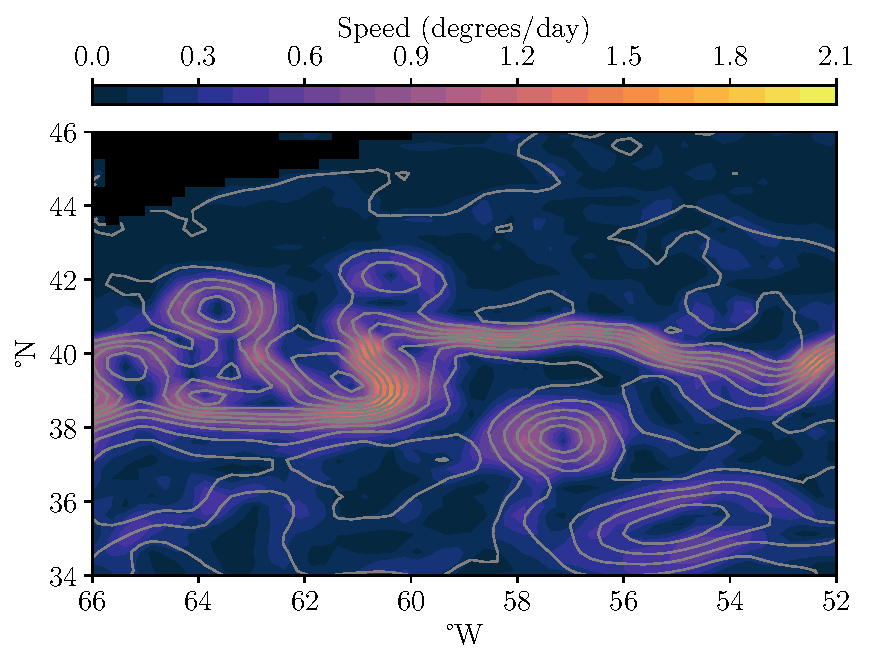
\includegraphics[width=\textwidth]{chp06_applications/figures/gulf_stream/streamlines_0}
% 			\caption{\(t = 0\) (midnight \DTMdisplaydate{2020}{01}{01}{})}
% 		\end{subfigure}
% 		\begin{subfigure}{0.49\textwidth}
% 			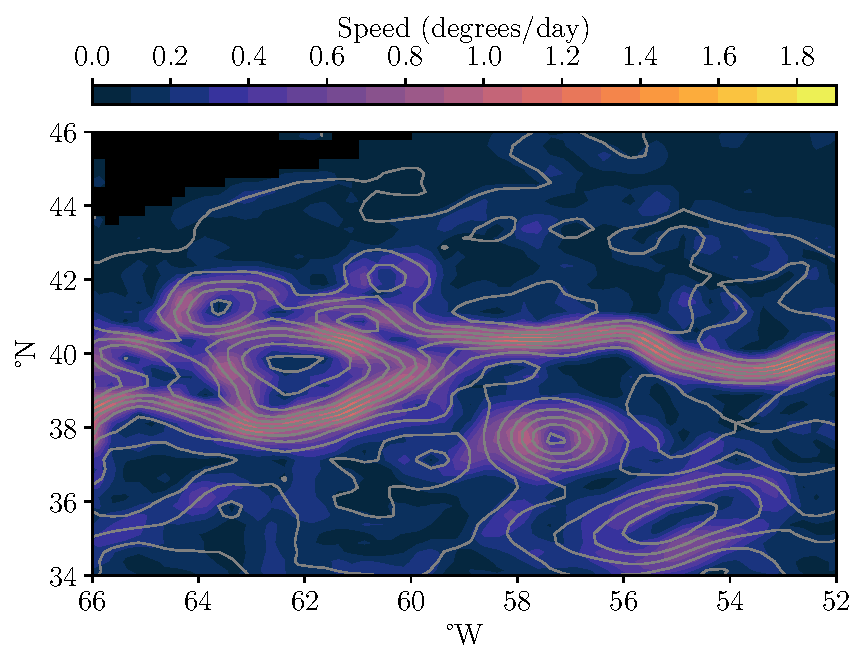
\includegraphics[width=\textwidth]{chp06_applications/figures/gulf_stream/streamlines_5}
% 			\caption{\(t = 5\) (midnight \DTMdisplaydate{2020}{01}{6}{})}
% 		\end{subfigure}
% 		\begin{subfigure}{0.49\textwidth}
% 			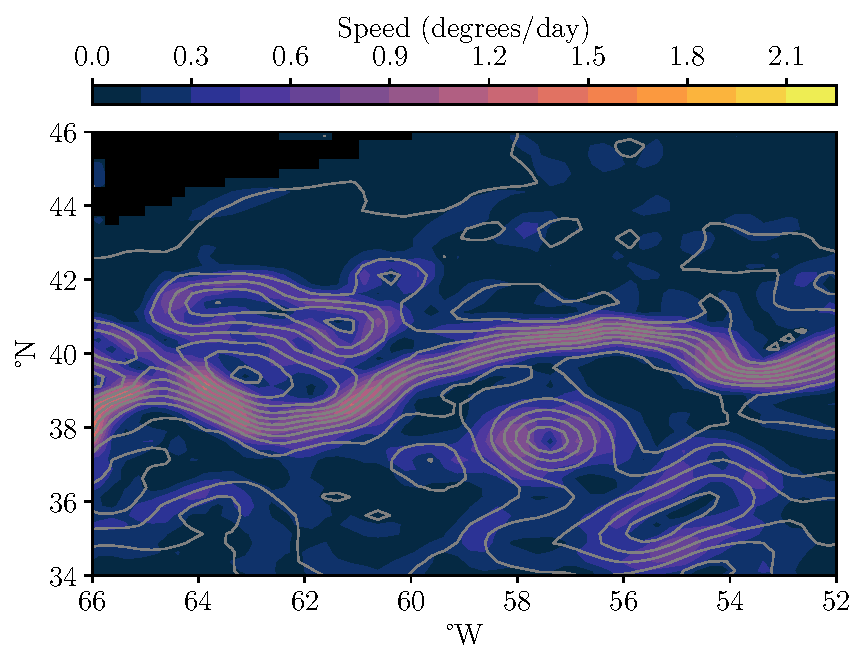
\includegraphics[width=\textwidth]{chp06_applications/figures/gulf_stream/streamlines_10}
% 			\caption{\(t = 10\) (midnight \DTMdisplaydate{2020}{01}{11}{})}
% 		\end{subfigure}
% 		\begin{subfigure}{0.49\textwidth}
% 			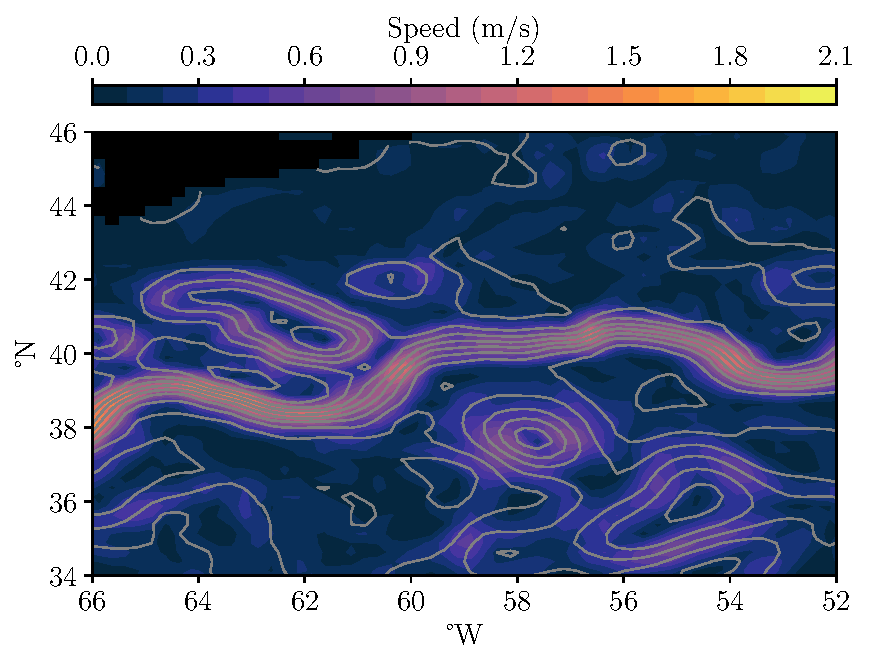
\includegraphics[width=\textwidth]{chp06_applications/figures/gulf_stream/streamlines_15}
% 			\caption{\(t = 15\) (midnight \DTMdisplaydate{2020}{01}{16}{})}
% 		\end{subfigure}
% 		\caption{The absolute surface current speed (coloured) and contours of the sea-surface height (streamlines of the flow, in grey) of the Gulf Stream dataset, at various times chosen to demonstrate the formation and separation of an eddy from the stream.
% 			The black region indicates missing data, due to the presence of land.
% 			All times are in Greenwich Mean Time.}
% 		\label{fig:na_motive_flow}
% 	\end{center}
% \end{figure}




The velocity data is Eulerian and unsteady (varying with time), so to predict the position of a drifter we must solve for a Lagrangian trajectory.
This requires interpolating the velocity data, for which we use a linear interpolate.
Let \(x_t \equiv \left(x_t^{(\mathrm{lon})}, x_t^{(\mathrm{lat})}\right)^{\T}\) denote the longitudinal and latitudinal position of the drifter \(t\) days after midnight \DTMdisplaydate{2020}{01}{01}{-1}.
The deterministic model for \(x_t\), constructed purely from the interpolated velocity data, is
\begin{equation}\label{eqn:natl_ode}
	\dod{}{t}\begin{bmatrix}
		x_t^{(\text{lon})} \\ x_t^{(\text{lat})}
	\end{bmatrix} = \begin{bmatrix}
		u\!\left(x^{(\mathrm{lon})}_t, x^{(\mathrm{lat})}_t, t\right) \\ v\!\left(x^{(\mathrm{lon})}_t, x^{(\mathrm{lat})}_t, t\right)
	\end{bmatrix},
\end{equation}
where \(u\) and \(v\) are the interpolated zonal and meridional velocities respectively.
In this context, we may think of \cref{eqn:natl_ode} as our ``best available'' deterministic model for the time-evolution of the drifter position; if the data (and the subsequent interpolation) were exactly correct, then \cref{eqn:natl_ode} would provide accurate predictions.
However, this is certainly not the case and there are many sources of uncertainty not accounted for by using \cref{eqn:natl_ode} alone.

\begin{figure}
	\centering
	\begin{subfigure}{0.49\textwidth}
		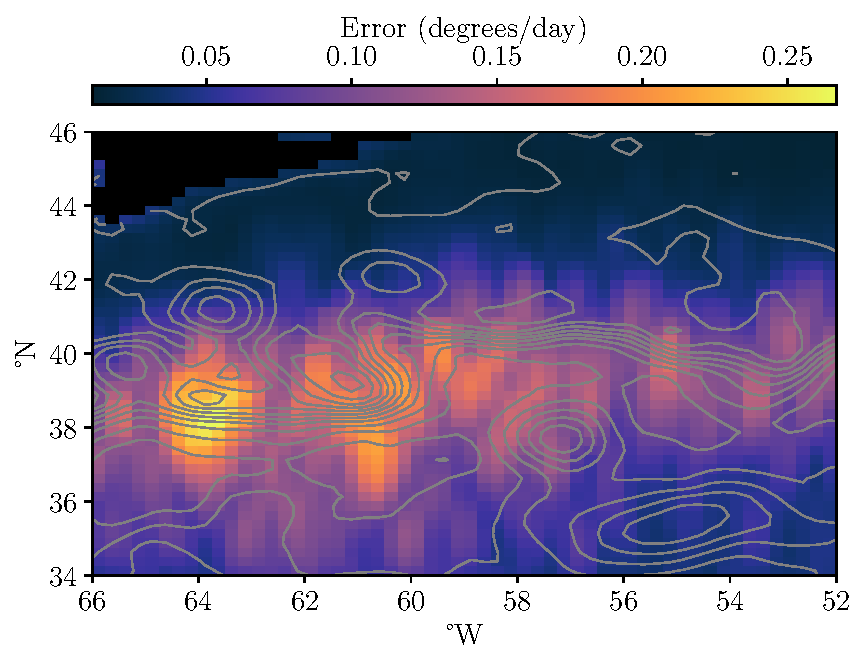
\includegraphics[width=\textwidth]{chp06_applications/figures/gulf_stream/u_err_0}
		\caption{Zonal component}
	\end{subfigure}
	\begin{subfigure}{0.49\textwidth}
		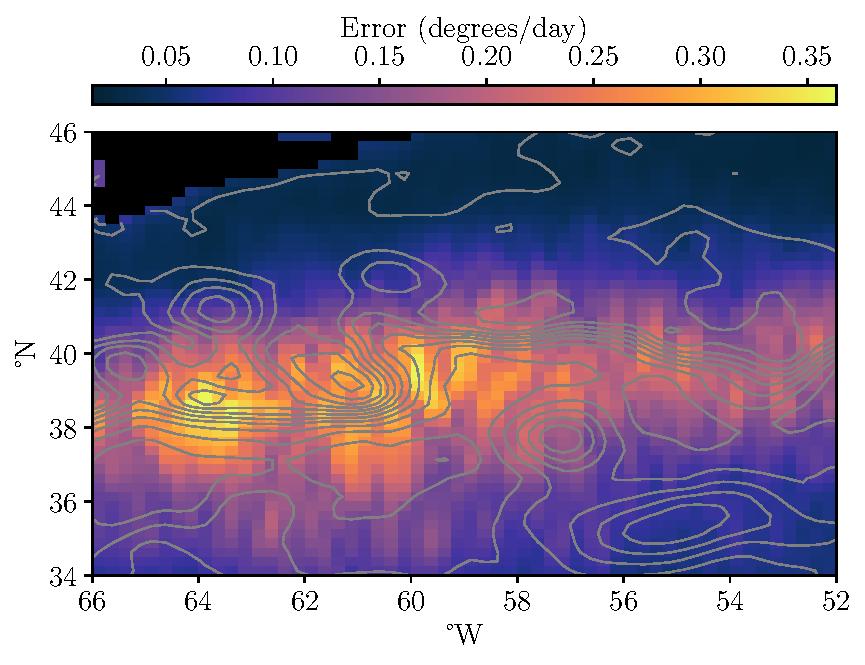
\includegraphics[width=\textwidth]{chp06_applications/figures/gulf_stream/v_err_0}
		\caption{Meridional component}
	\end{subfigure}
	\caption{The mapping error in the (a) zonal (longitudinal) and (b) meridional velocity components at midnight \DTMdisplaydate{2020}{01}{01}{-1}.}
	\label{fig:natl_err}
\end{figure}

The dataset additionally includes estimates for the mapping error (an estimate of the variance) in the zonal and meridional velocity measurements, and in particular provides an indication of measurement error; typically the error is smaller in regions directly under satellite tracks.
The mapping error in each velocity component at \(t = 0\) is shown in \Cref{fig:natl_err}, as an example of the structure of the field, along with contours of the sea surface height.
The error varies with time, but retains the main structure in which is appears highest along the Gulf Stream, which is not a surprise as this region contains the most complicated part of the flow.
We can capture both the spatial and temporal variation in this mapping error by adding multiplicative noise to the deterministic model \cref{eqn:natl_ode}.
To account for measurement error, we use the following stochastic model:
\begin{equation}
	\dif \begin{bmatrix}
		x^{(\mathrm{lon})}_t \\ x^{(\mathrm{lat})}_t
	\end{bmatrix} = \begin{multlined}[t]
		\begin{bmatrix} u\left(x^{(\mathrm{lon})}_t, x^{(\mathrm{lat})}_t, t\right) \\ v\left(x^{(\mathrm{lon})}_t, x^{(\mathrm{lat})}_t, t\right) \end{bmatrix}\dif t \\
		+ L_r\begin{bmatrix}
			\sqrt{u_{\mathrm{err}}\left(x^{(\mathrm{lon})}_t, x^{(\mathrm{lat})}_t, t\right)} & 0                                                                                 \\
			0                                                                                 & \sqrt{v_{\mathrm{err}}\left(x^{(\mathrm{lon})}_t, x^{(\mathrm{lat})}_t, t\right)}
		\end{bmatrix} \dif W_t,
	\end{multlined}
	\label{eqn:natl_sde}
\end{equation}
where \(u_{\mathrm{err}}\) and \(v_{\mathrm{err}}\) are the interpolated error estimates for the zonal and meridional velocities (converted to \unit{\degree\per\square\day} using the same transformation as was done on the velocity data), and \(L_r = 0.25 \mathrm{\,degrees}\) is the spatial resolution of the data.



% The derivatives \(\nabla u\) of the deterministic velocity field in \cref{eqn:natl_sde} are approximated via the centred finite-differences,
% \begin{align*}
% 	\dpd{u\left({x^{(\text{lon})}}, {x^{(\text{lat})}}, t\right)}{{x^{(\text{lon})}}} & \approx \frac{u\left(x^{(\text{lon})} + L_r, x^{(\text{lat})}, t\right) - u\left(x^{(\text{lon})} - L_r, x^{(\text{lat})}, t\right)}{2 L_r},
% \end{align*}
% and similar for the remaining derivatives.



% We will now introduce an example of a differential equation model constructed from observed data, which we will use throughout this chaper, and explore further in \Cref{ch:appls}.
% In particular, the technical details of this example will be provided in \Cref{sec:appl_ocean}.

% Suppose we are interested in tracking the position of a drifter on the surface of the Gulf Stream.
% The only information we have available are measurements of the eastwards (zonal) and northwards (meridional) velocities at the surface, derived from altimetry (sea surface height) data.
% Such data is available from the European Commission`s Copernicus Marine Environment Monitoring Service.

% For the purposes of this example, assume that the position of the drifter at the initial time is known exactly\footnote{In practice, of course, this will not be the case, but this will introduce even more uncertainty into our model, furthering reinforcing the purpose of this example.}.
% Assuming that the interpolated data provided an accurate model of the sea surface velocity, the position \(x_t\) of the drifter on the surface at time \(t\) is the solution to the ordinary differential equation
% \begin{equation}\label{eqn:na_motiv_ode}
% 	\dod{x_t}{t} = u\left(x_t, t\right),
% \end{equation}
% subject to the known initial position \(x_0\), where \(u\) is the appropriately interpolated surface velocity data.
% To illustrate the time-varying dynamics of the Stream, \Cref{fig:na_motiv_flow} plots contours the sea-surface height, which correspond to the time-varying streamfunction of the flow, and therefore solutions to \cref{eqn:na_motiv_ode}, at various times.
% An important feature of the flow is that there are significantly different qualitative regimes; there is the rapidly moving stream itself, the eddies that are shed and slow moving, and isotropic regions in between where the current is comparatively slow.



% We can easily solve \cref{eqn:na_motiv_ode} numerically to obtain a predicted position for our drifter on day \(t\).
% % We term \cref{eqn:na_motiv_ode} the \emph{deterministic model}, since given the data we have available, it serves as our best purely deterministic model for the position of the drifter.
% Suppose that our drifter begins within the stream itself, at \(x_0 = \left(-60.5, 39\right)^{\T}\), \Cref{fig:na_motiv_det} plots the resulting trajectory (in white) obtained by solving \cref{eqn:na_motiv_ode} numerically, over the span of 7 days starting from midnight \DTMdisplaydate{2020}{01}{01}{}.
% Based on this model, we expect that the drifter will follow the Stream, which can inform efforts to locate the drifter.

% \begin{figure}
% 	\begin{center}
% 		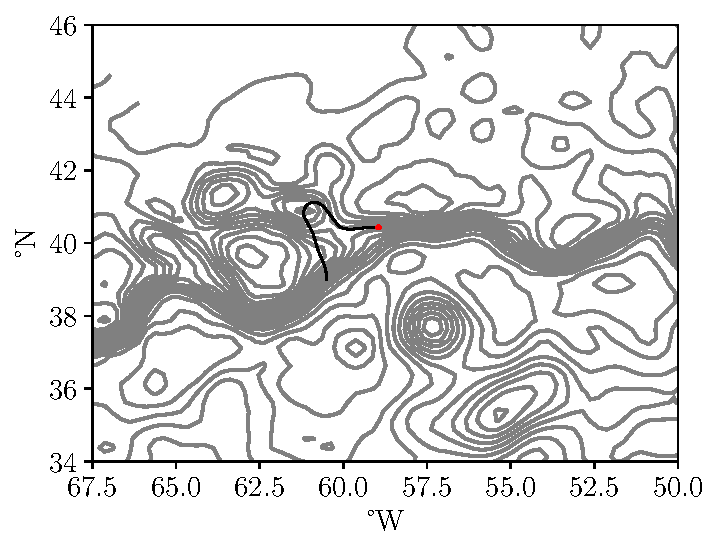
\includegraphics[width=\textwidth]{chp06_applications/figures/gulf_stream_motivation/det_traj.pdf}
% 		\caption{The time evolution of the solution (obtained by numerically integrating the velocity data) to the deterministic system corresponding to \cref{eqn:natl_sde}, from initial condition \(x_0 = \left(-60.5, 39\right)^{\T}\) from 01/01/2021 (\(t = 0\)) to 08/01/2021 (\(t = 8\)).
% 			Contours of the sea surface height at the final time \(t = 8\) are included in grey to indicate the position of the Gulf Stream and nearby eddies in the flow.}
% 		\label{fig:na_motiv_det}
% 	\end{center}
% \end{figure}

% To improve our predictions of the future position of the drifter, we should attempt to account for this uncertainty in our model \cref{eqn:na_motiv_ode}.
% The altimetry-derived data also includes measures of error in each component of the velocity at each spatiotemporal gridpoint, so we can use these measurements to model the ongoing observational error in \(u\).
% We can extend \cref{eqn:na_motiv_ode} as a stochastic differential equation, where the unresolved uncertainty is parameterised as a white-noise process scaled by measurement error.
% Specifically, we formulate the drifter position as \cref{eqn:natl_sde} in \Cref{sec:gulf_stream}, which is explained in more detail in that section.
% For our purposes here, \cref{eqn:natl_sde} is a stochastic differential equation analogy of \cref{eqn:natl_sde} that we can solve numerically to obtain approximate solution samples.

% \Cref{fig:na_motiv_rels} shows us the result of numerically solving a stochastic differential equation formulation (specifically ) of the Lagrangian trajectory model.
% This is a ``more correct'' model than the deterministic counterpart, in the sense that it is attempting to account for the unknowable measurement error and unresolved subgrid effects.
% Each realisation here could correspond to our drifter, and we see a far different picture than the deterministic model alone provided.
% Qualitatively, rather than following the Stream itself, a proportion of particles are caught in one of two eddies which have formed and broken off from the Stream.

% \begin{figure}
% 	\begin{center}
% 		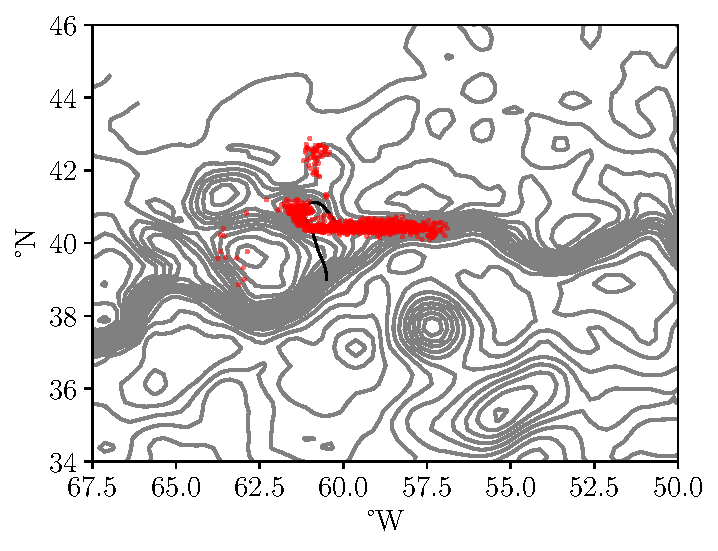
\includegraphics[width=\textwidth]{chp06_applications/figures/gulf_stream_motivation/num_rels.pdf}
% 		\caption{The same visualisation of the deterministic behaviour of the Gulf Stream example as \Cref{fig:na_motive_det}, but with the final positions of 10000 numerical realisations of a stochastic model, each indicated by a red point.}
% 		\label{fig:na_motiv_rels}
% 	\end{center}
% \end{figure}

% Although deterministic models are often easier to work with analytically and far more efficient to solve numerically, these models are limited.
% By explicitly accounting for uncertainty with a stochastic, we can expand the scope of our model and provide more realistic and useful predictions, at the cost of a more complicated model.
% This idea of introducing stochastic components into a deterministic model to account for unresolved and unknown aspects has been used extensively in recent times across scientific applications, notably atmospheric, climate, and oceanographic modelling.
% We provide an overview of this so-called stochastic parameterisation in the next section, and highlight how the work of this thesis fits in with the needs of that field.



\subsection{Exploring a single trajectory}
In this example, we shall consider a fixed initial condition and explore the resulting trajectory.
Suppose that at midnight \DTMdisplaydate{2021}{01}{01}{-1}, the drifter is located within the stream  at longitude \(60.5^\circ\) west and \(39^\circ\) north.
We accordingly consider the evolution of the models \cref{eqn:natl_ode} and \cref{eqn:natl_sde} with the initial condition \(x_0 = (-60.5, 39)^{\T}\).
By solving the deterministic model \cref{eqn:natl_ode} numerically, we predict the position of the drifter after \(t = 7\) days (at midnight \DTMdisplaydate{2021}{01}{08}{-1}) and show the time-evolution of the solution trajectory in \Cref{fig:natl_det_traj}.
The drifter is transported by the jet stream.
This is the prediction of the deterministic model \cref{eqn:natl_ode}, but when accountinf for uncertainty with the stochastic model \cref{eqn:natl_sde}, we get a more complicated picture.
\Cref{fig:natl_stoch_rels} shows the result of \(N = 1000\) numerical realisations (obtained via Euler-Maruyama integration with a step size of ) of the stochastic model \cref{eqn:natl_sde}, starting from the fixed initial condition \(x_0\) and evolved over the same week-long time frame.
Each red point corresponds to a single realisation at midnight \DTMdisplaydate{2021}{01}{08}{-1}; although a large number of the realisations have been transported along the stream, many break off from the stream in eddies, resulting in several clusters.
This example highlights the importance of stochastic models; the deterministic model suggests that the drifter will follow the Stream itself, but the dynamic behaviour of the flow means that any stochasticity can result in vastly different positions.

\begin{figure}
	\begin{center}
		\begin{subfigure}[t]{0.49\textwidth}
			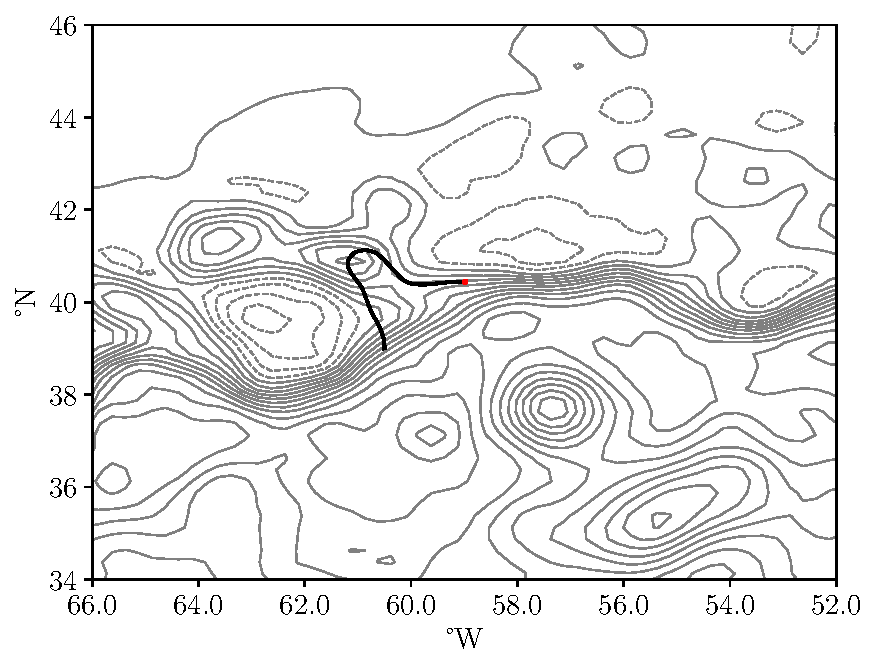
\includegraphics[width=\textwidth]{chp06_applications/figures/gulf_stream/det_traj.pdf}
			\caption{The solution to the deterministic model \cref{eqn:natl_ode}.}
			\label{fig:natl_det_traj}
		\end{subfigure}
		\begin{subfigure}[t]{0.49\textwidth}
			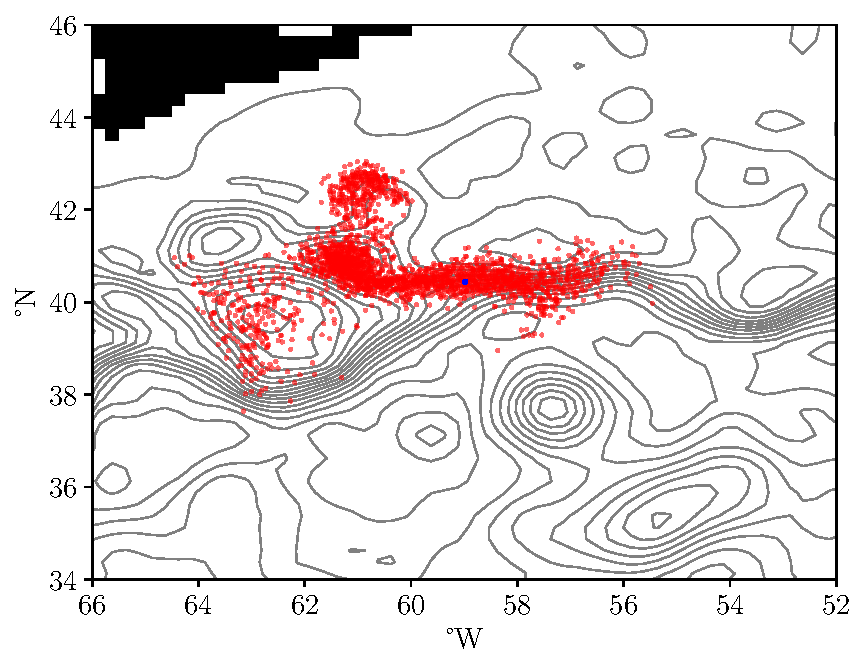
\includegraphics[width=\textwidth]{chp06_applications/figures/gulf_stream/traj_stoch_rels}
			\caption{Numerical realisations of the solution to the stochastic model \cref{eqn:natl_sde}.}
			\label{fig:natl_stoch_rels}
		\end{subfigure}
		\caption{Solutions to the deterministic model \cref{eqn:natl_ode} in (a) and stochastic model \cref{eqn:natl_sde} in (b) for fixed initial condition \((-60.5, 39)^{\T}\) from midnight \DTMdisplaydate{2021}{01}{01}{-1} to midnight \DTMdisplaydate{2021}{01}{08}{-1}, corresponding to a drifter on the surface of the Gulf Stream.
			The deterministic prediction at the final time is indicated in blue in both figures, with the time evolution of the deterministic trajectory in black in (a).
			In (b), each red point corresponds to one of 2500 realisations of the stochastic solution at midnight \DTMdisplaydate{2021}{01}{08}{-1}.
			Contours of the sea surface height at the final time are included in grey, which correspond to contours of the streamfunction at that time.
			The regions of land for which there is no data is indicated in black.}
	\end{center}
\end{figure}

\begin{figure}
	\begin{center}
		\begin{subfigure}{0.49\textwidth}
			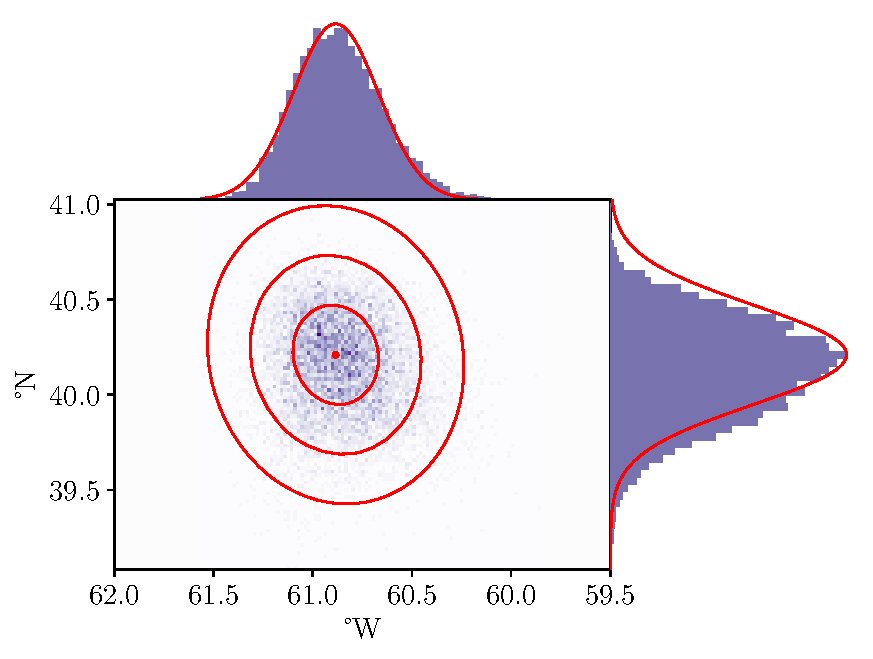
\includegraphics[width=\textwidth]{chp06_applications/figures/gulf_stream/traj_stoch_em_1.0}
			\caption{\(t = 1\) (midnight \DTMdisplaydate{2021}{02}{01}{-1}))}
		\end{subfigure}
		\begin{subfigure}{0.49\textwidth}
			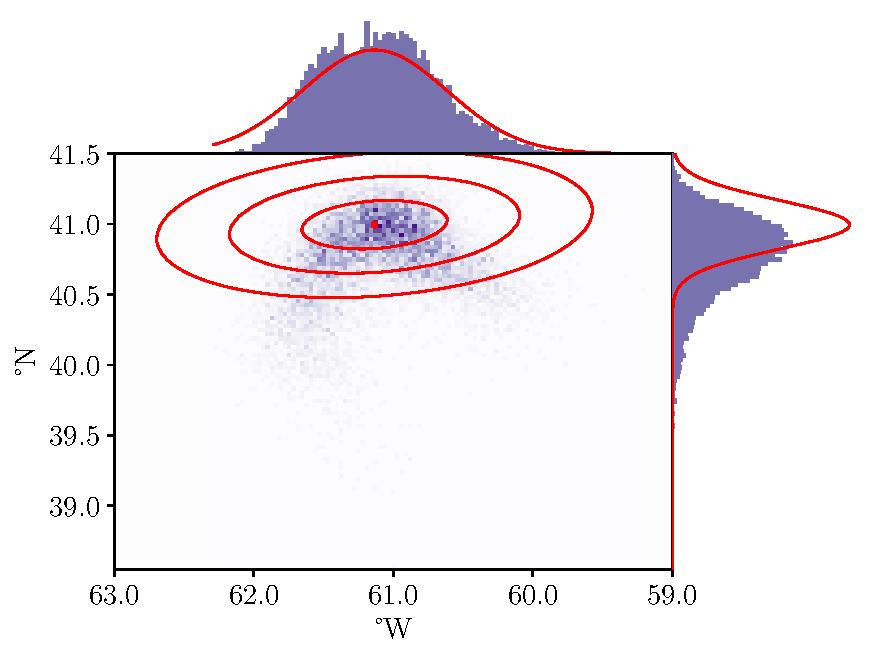
\includegraphics[width=\textwidth]{chp06_applications/figures/gulf_stream/traj_stoch_em_2.0}
			\caption{\(t = 2\) (midnight \DTMdisplaydate{2021}{05}{01}{-1}))}
		\end{subfigure}
		\begin{subfigure}{0.49\textwidth}
			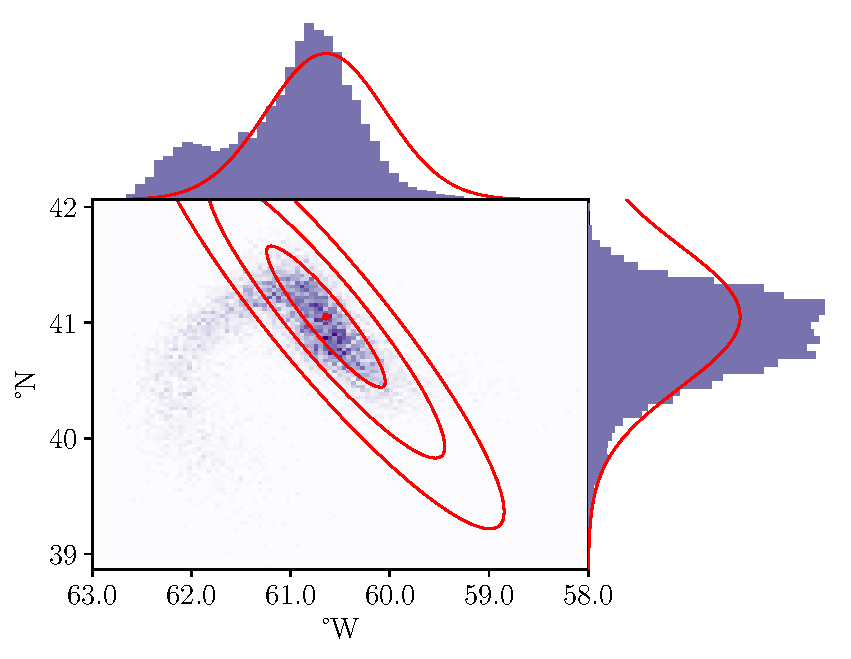
\includegraphics[width=\textwidth]{chp06_applications/figures/gulf_stream/traj_stoch_em_3.0}
			\caption{\(t = 3\) (midnight \DTMdisplaydate{2021}{08}{01}{-1}))}
			\label{fig:natl_em_3}
		\end{subfigure}
		\begin{subfigure}{0.49\textwidth}
			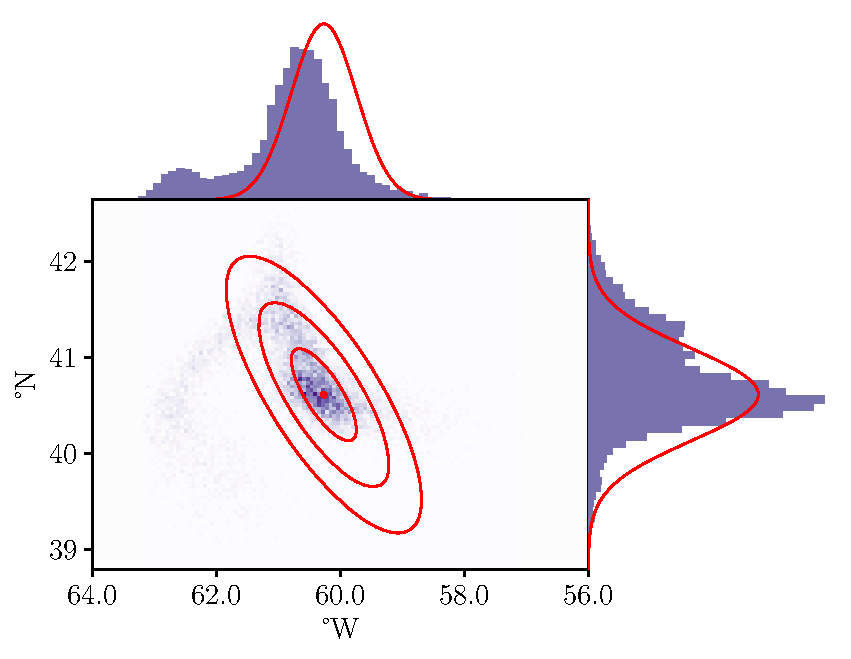
\includegraphics[width=\textwidth]{chp06_applications/figures/gulf_stream/traj_stoch_em_4.0}
			\caption{\(t = 4\) (midnight \DTMdisplaydate{2021}{08}{01}{-1}))}
		\end{subfigure}
		\begin{subfigure}{0.49\textwidth}
			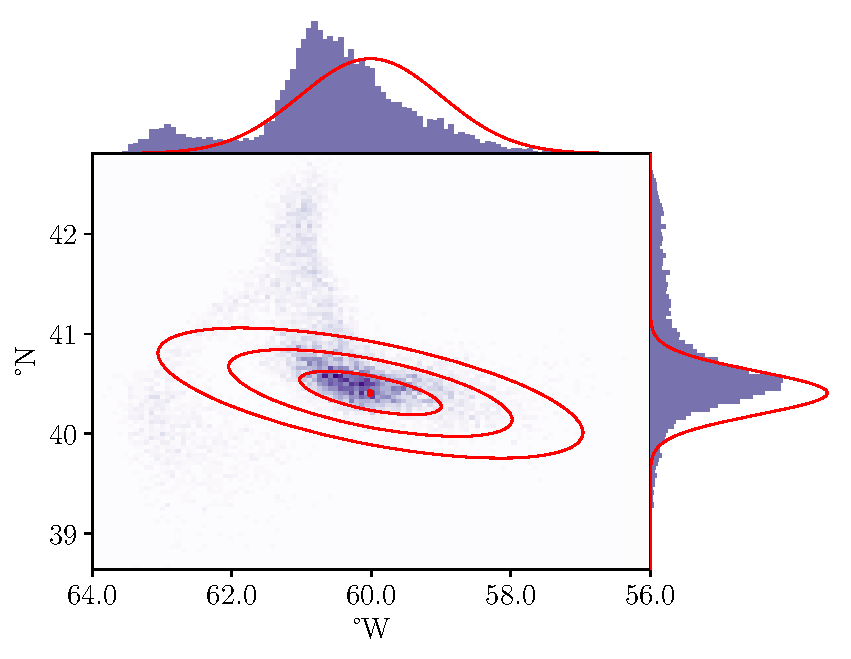
\includegraphics[width=\textwidth]{chp06_applications/figures/gulf_stream/traj_stoch_em_5.0}
			\caption{\(t = 5\) (midnight \DTMdisplaydate{2021}{08}{01}{-1}))}
		\end{subfigure}
		\begin{subfigure}{0.49\textwidth}
			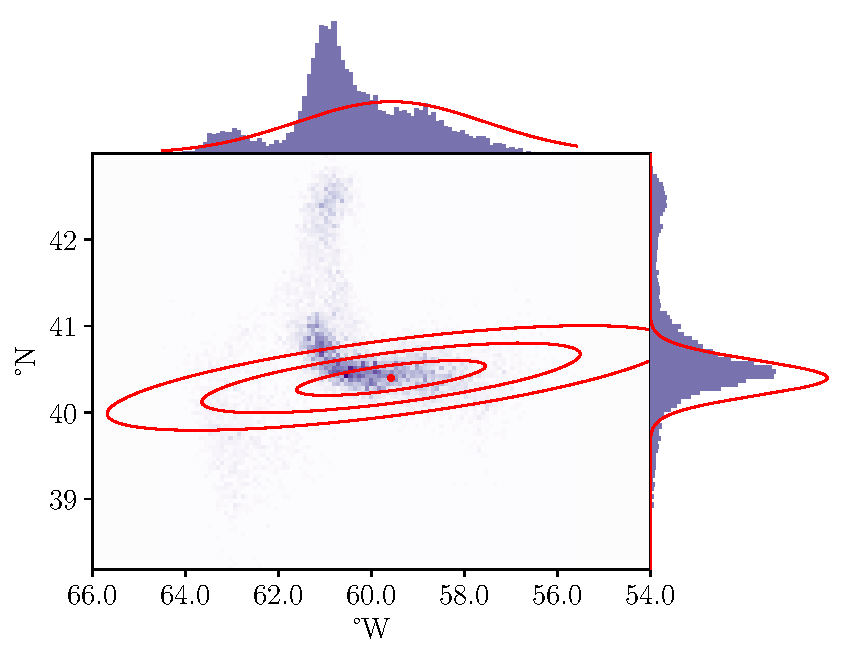
\includegraphics[width=\textwidth]{chp06_applications/figures/gulf_stream/traj_stoch_em_6.0}
			\caption{\(t = 6\) (midnight \DTMdisplaydate{2021}{08}{01}{-1}))}
		\end{subfigure}
		\caption{The time-evolution of \(N = 10000\) Euler-Maruyama realisations of the solution to \cref{eqn:natl_sde}, with the Gaussian density arising from a linearisation of \cref{eqn:natl_sde} about the deterministic trajectory overlaid in red.
			The bivariate plot shows contours of the probability density function (or equivalently standard deviation bounds) of the Gaussian approximation, whereas each marginal plot on the longitudinal and latitudinal axis show the PDFs themselves of the Gaussian marginals.}
		\label{fig:natl_em}
	\end{center}
\end{figure}

We now move onto a more precise analysis of the time-evolution probability distribution of this solution to the stochastic model \cref{eqn:natl_sde}, and apply the tools we have developed in \Cref{ch:linear_theory,ch:gmm}.
\Cref{fig:natl_em} shows histograms of \(N = 10000\) Euler-Maruyama samples at various times between \DTMdisplaydate{2021}{01}{01}{-1} and \DTMdisplaydate{2021}{01}{08}{-1}.
The marginal distributions in the longitudinal and latitudinal directions are shown on each axis.
Overlaid in red are the Gaussian solution to the linearisation of \cref{eqn:natl_sde}, computed by numerically solving the ODE \cref{eqn:pi_ode} for the covariance matrix.
The deterministic trajectory and covariance matrix are computed simultaneously using the Mazzoni method outlined in \Cref{sec:mazzoni}.
This computation requires the gradient of the velocity field, which we approximate with a centered finite difference.
In \Cref{fig:natl_em}, on each joint histogram we have plotted contours of the bivariate Gaussian, and on each marginal we have plotted the probability density function of the Gaussian solution corresponding to that component.
\td{Interpret the plots. Nothing too crazy to say. Need to make sure they are actually correct, however. \(t = 1\) not looking great.}
After a single day (\(t = 1\)), the numerical realisations match the Gaussian approximation.
The distribution is clearly non-Gaussian, due to both the nonlinearity of the flow and the multiplicative noise introduced by the measurement errors.



\begin{figure}
	\begin{center}
		% \begin{subfigure}[t]{0.49\textwidth}
		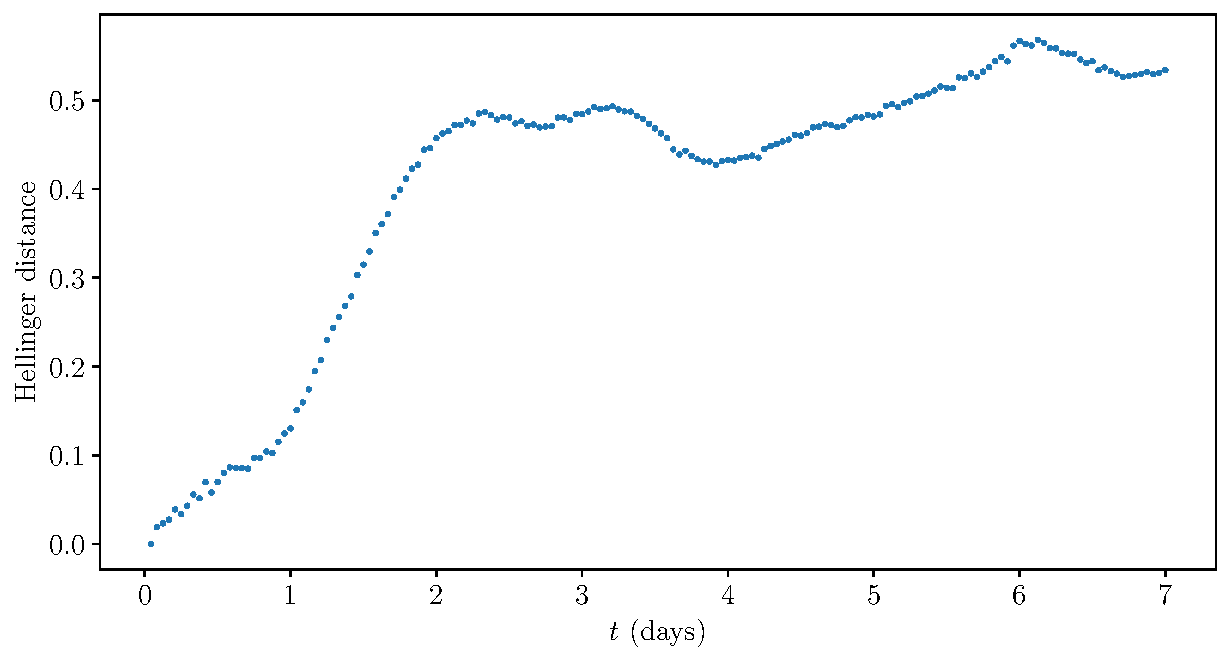
\includegraphics[width=\textwidth]{chp06_applications/figures/gulf_stream/traj_stoch_hell_dist_0.25}
		\caption{The estimated Hellinger distance between \(N = 10000\) Euler-Maruyama samples of \cref{eqn:natl_sde} and the Gaussian process solution to the linearisation, \(t\) days after midnight \DTMdisplaydate{2021}{01}{01}{-1}.}
		\label{fig:natl_hell}
		% \end{subfigure}
		% \begin{subfigure}[t]{0.49\textwidth}
		% 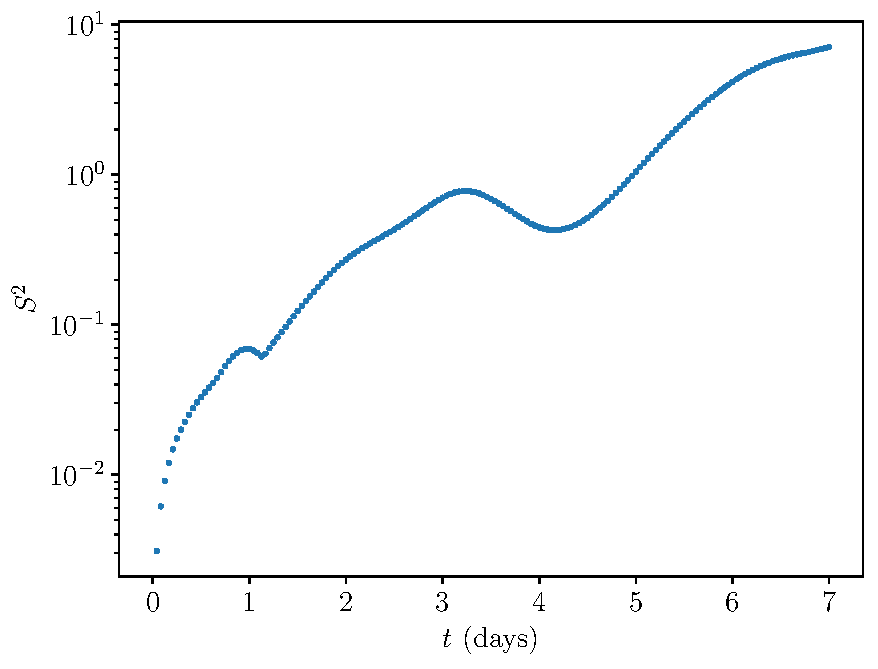
\includegraphics[width=\textwidth]{chp06_applications/figures/gulf_stream/traj_stoch_S2}
		% 	\caption{Stochastic sensitivity \(S^2\).}
		% \end{subfigure}
		% \begin{subfigure}[t]{0.49\textwidth}
		% 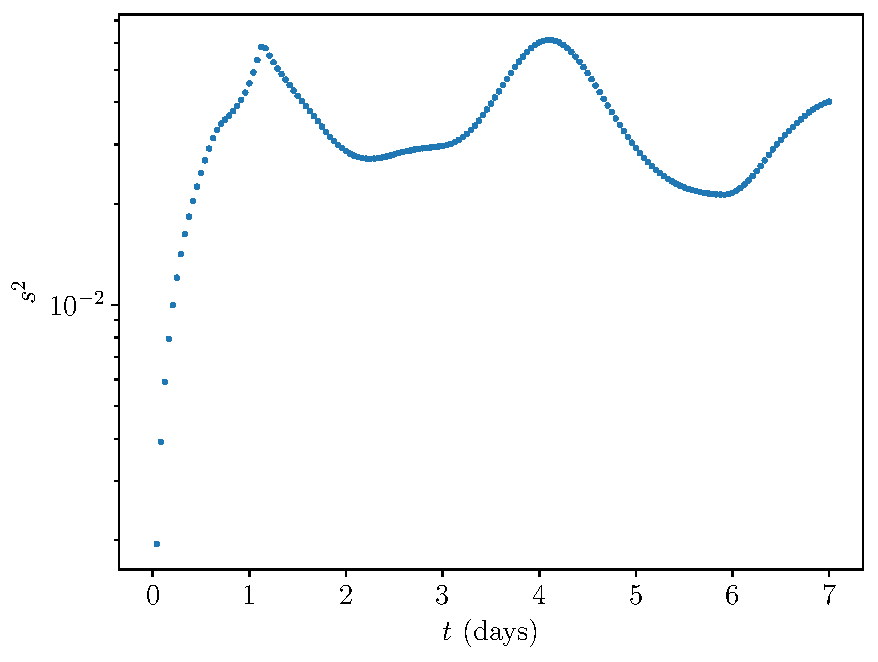
\includegraphics[width=\textwidth]{chp06_applications/figures/gulf_stream/traj_stoch_s2min}
		% 	\caption{The minimum eigenvalue of the linearisation covariance matrix.}
		% \end{subfigure}
		% \begin{subfigure}[t]{0.49\textwidth}
		% 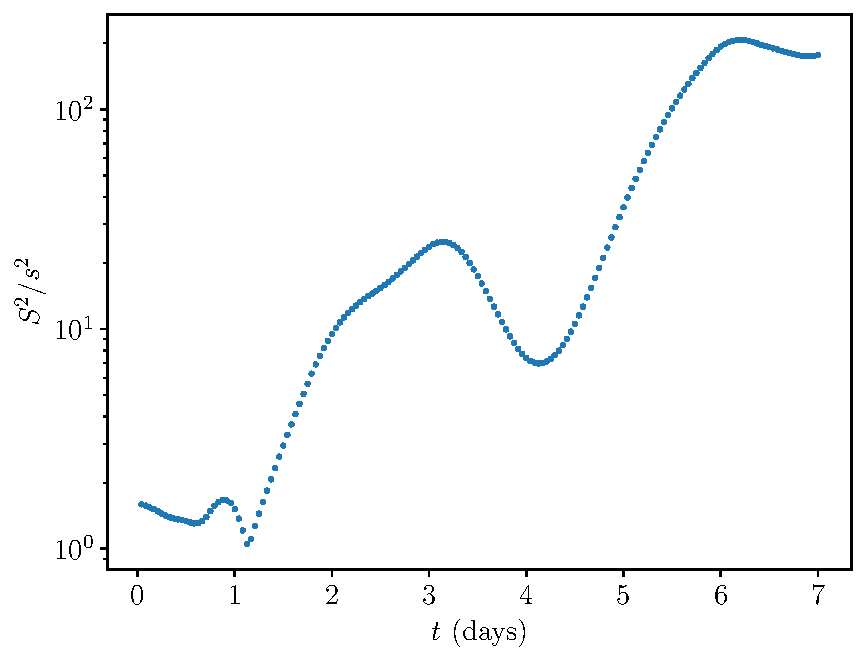
\includegraphics[width=\textwidth]{chp06_applications/figures/gulf_stream/traj_stoch_ratio}
		% 	\caption{The ratio of eigenvalues of the linearisation covariance matrix.}
		% \end{subfigure}
		% \caption{ \(t\) days after midnight \DTMdisplaydate{2021}{01}{01}{-1}.}
		% \label{fig:natl_metrics}
	\end{center}
\end{figure}

To evaluate the Gaussian approximation over
\Cref{fig:natl_hell} plots the Hellinger distance between the Gaussian approximation and Euler-Maruyama samples solving \eqref{eqn:natl_sde}, using a bin size corresponding to the .
In \Cref{app:supp_hell_natl}, we provide additional figures showing the same computation, but for varying bin sizes, to verify that the Hellinger distance computation is reasonably robust to changes in this size.
\td{Actually get this plots in there.}
As expected, the distance increases over time, as the numerical solution to \eqref{eqn:natl_sde} quickly becomes non-Gaussian.
However, there are two times where the Gaussian approximation \emph{improves}: at \(t \approx 3.3\) and \(t \approx 6\).



\td{Conclude by answering `so what?`. Why would we want such approximations in the first place? How is this any better? We just have a shit approximation of a highly non-Gaussian distribution.}


\subsection{Stochastic sensitivity}
As in \Cref{sec:comput_s2} of \Cref{ch:linear_numerics}, the purpose of this example is to demonstrate the computation of stochastic sensitivity from the covariance matrix, rather than provide any new insight.
A similar example of computing the stochastic sensitivity field for a similar sea-surface dataset of the Gulf Stream, albeit using the original method of calculation \citep{Balasuriya_2020_StochasticSensitivityComputable}, is found in \citet{BadzaEtAl_2023_HowSensitiveAre}.

\Cref{fig:na_s2_grid} plots the stochastic sensitivity field for a grid of initial conditions at the \(0.25^\circ \times 0.25^\circ\) resolution of the velocity data.
That is, each initial condition corresponds to a point at which the surface velocity data was available.


The stream is outlined by regions of high uncertainty, which is expected as near these edges trajectories can undergo qualitatively very different behaviours by either remaining in the stream or leaving it in an eddy.

Away from the stream (either north or south of it), the flow is reasonably isotropic and the level of noise from measurement error is small and consequently there is a relatively small uncertainty in the trajectories.

At higher resolutions, conclusions from the deterministic model alone cannot be trusted completely; between the gridpoints the velocity data has been interpolated.
Although the stochastic model also uses this interpolated data, the fact that the model can account
This is an advantage of stochastic sensitivity over other deterministic measures, such as the finite-time Lyapunov exponent, which are limited by the resolution of the data.




On the right-hand side of \Cref{fig:na_s2}, we show robust sets extracted from the stochastic sensitivity field at each resolution, using a threshold of \(2^\circ\).
Additional plots showing robust sets extracted with different thresholds are provided in \Cref{app:s2_robust}, and result in \td{something}.
...
This structure is better resolved in the higher-resolution field, where we can clearly see
The centres of these vortices, where we expect coherency in the deterministic system, and therefore robustness in the stochastic system, are also included in the set.



\begin{figure}
	\centering
	\begin{subfigure}{\textwidth}
		\includegraphics[width=0.49\textwidth]{chp06_applications/figures/gulf_stream/S2_field_grid}
		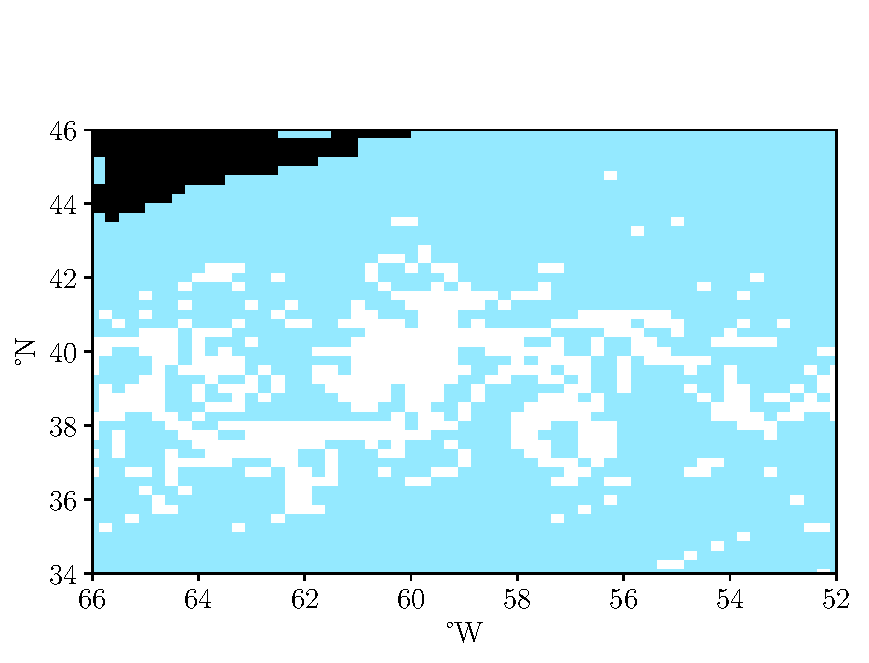
\includegraphics[width=0.49\textwidth]{chp06_applications/figures/gulf_stream/S2_robust_grid_2.0}
		\caption{At the \(0.25^\circ \times 0.25^\circ\) resolution of the velocity data.}
		\label{fig:na_s2_grid}
	\end{subfigure}
	\begin{subfigure}{\textwidth}
		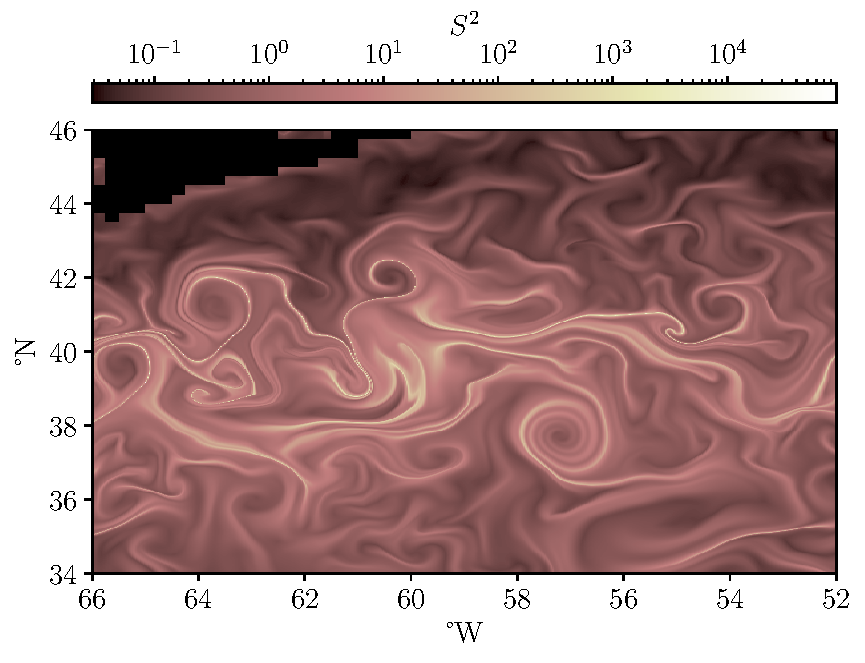
\includegraphics[width=0.49\textwidth]{chp06_applications/figures/gulf_stream/S2_field_high}
		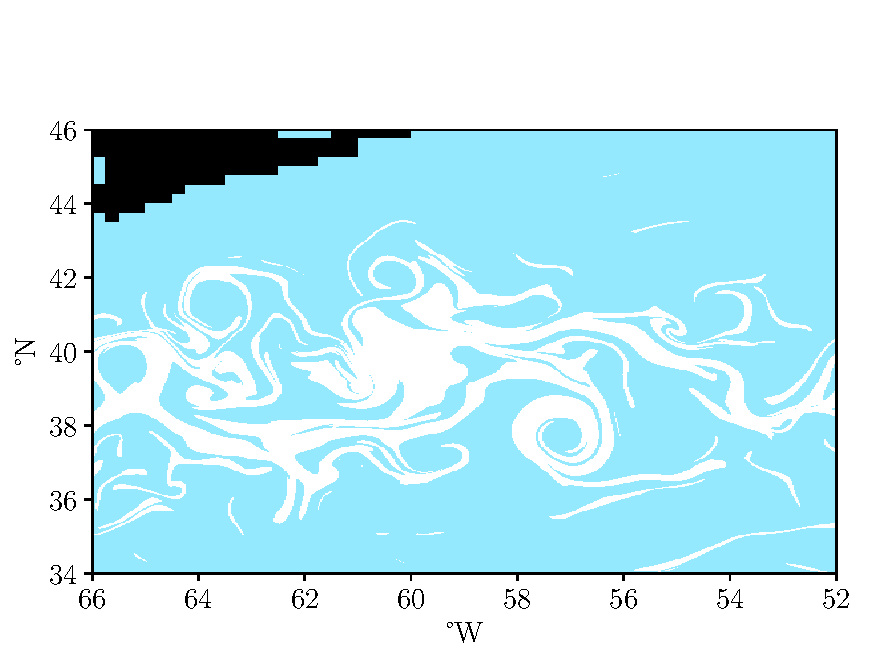
\includegraphics[width=0.49\textwidth]{chp06_applications/figures/gulf_stream/S2_robust_high_2.0}
		\caption{At the higher resolution of \(0.025^\circ \times 0.025^\circ\).}
		\label{fig:na_s2_grid}
	\end{subfigure}
	% \begin{subfigure}[t]{0.49\textwidth}
	% 	\includegraphics[width=\textwidth]{chp06_applications/figures/gulf_stream/S2_field_grid}
	% 	\caption{The stochastic sensitivity \(S^2\).}
	% 	\label{fig:na_S2}
	% \end{subfigure}
	% \begin{subfigure}[t]{0.49\textwidth}
	% 	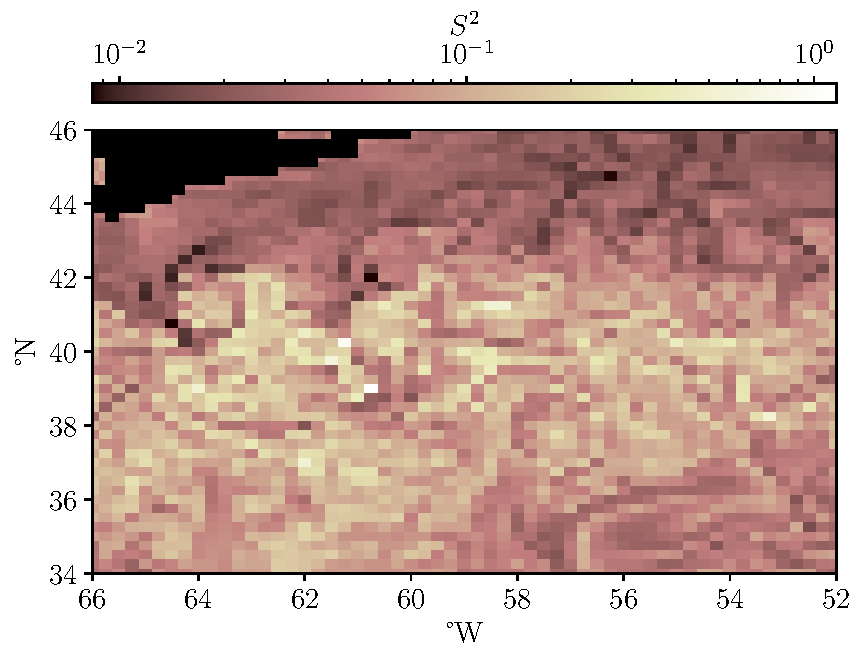
\includegraphics[width=\textwidth]{chp06_applications/figures/gulf_stream/s2min_field_grid}
	% 	\caption{The minimum eigenvalue of the covariance matrix.}
	% \end{subfigure}
	% \begin{subfigure}[t]{0.49\textwidth}
	% 	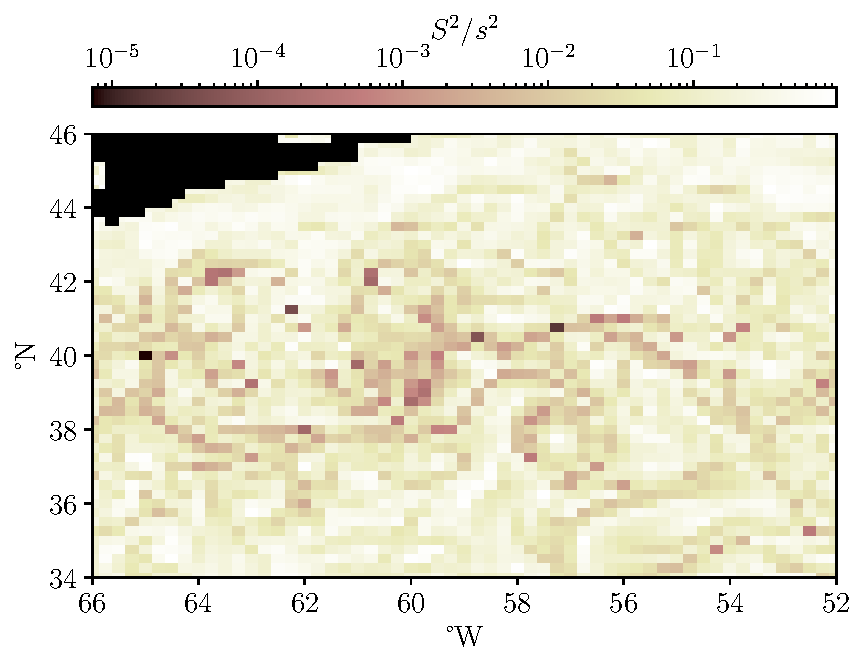
\includegraphics[width=\textwidth]{chp06_applications/figures/gulf_stream/ratio_field_grid}
	% 	\caption{The ratio of the stochastic sensitivity value (maximum eigenvalue) and the minimum eigenvalue of the covariance matrix, which captures the `narrowness' of the linearised distribution.}
	% \end{subfigure}
	% \begin{subfigure}[t]{0.49\textwidth}
	% 	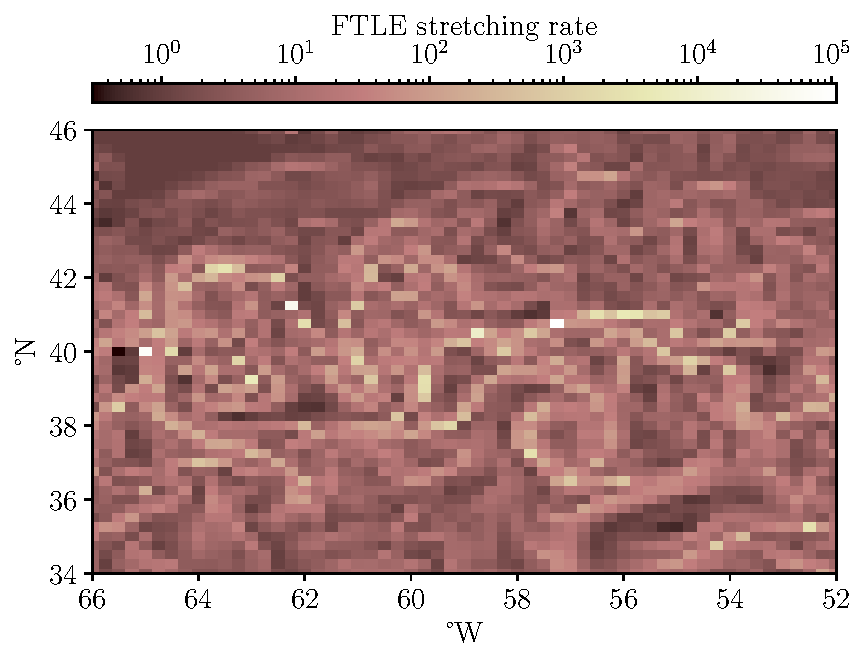
\includegraphics[width=\textwidth]{chp06_applications/figures/gulf_stream/ftle_field_grid}
	% 	\caption{The stretching rate field used in the FTLE calculation.}
	% \end{subfigure}
	% \begin{subfigure}[t]{0.49\textwidth}
	% 	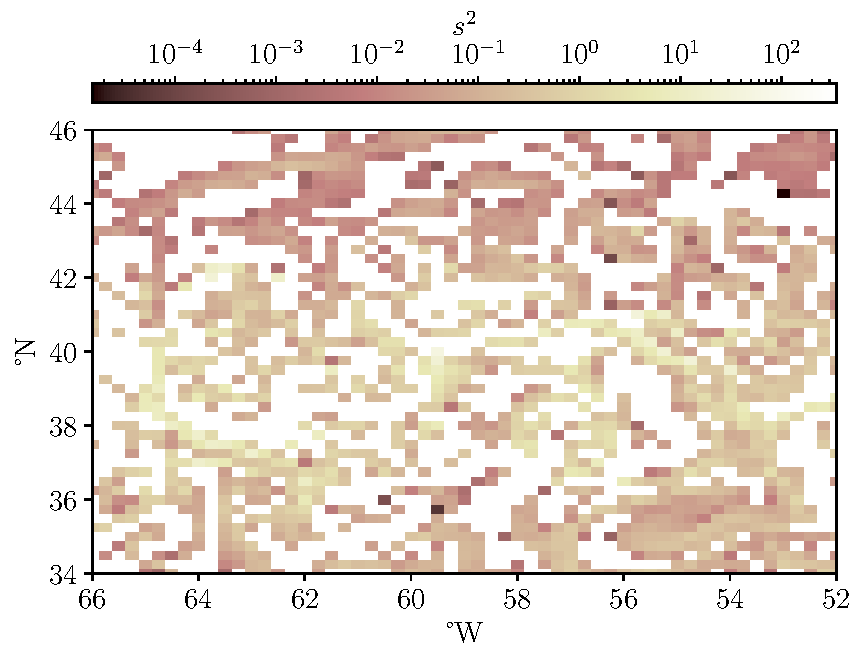
\includegraphics[width=\textwidth]{chp06_applications/figures/gulf_stream/cov_field_grid}
	% 	\caption{The \((1,2)\)th entry of the covariance matrix, corresponding to the covariance between coordinates.
	% 		White indicates regions in which the entry is zero.}
	% \end{subfigure}
	\caption{The stochastic sensitivity fields (left) computed from the linearisation covariance matrix on a grid of initial conditions, at two different resolutions.
		Note that values near the boundaries of the data and the land are not trustworthy, as the Gaussian approximations do not account for these boundaries.
		From each field, robust sets corresponding to coherent structures are extracted with a threshold of \(R = 2^\circ\) and shown on in cyan the right.
		In all figures, the regions of land for which there is no velocity data is indicated in black.}
	\label{fig:na_s2}
\end{figure}






% \begin{figure}
% 	\begin{center}
% 		\begin{subfigure}[t]{\textwidth}
% 			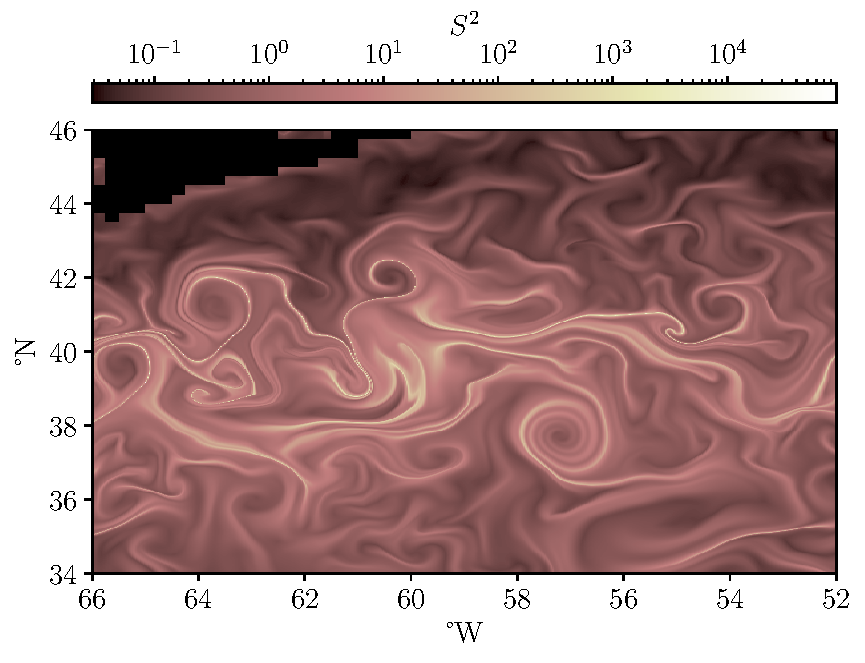
\includegraphics[width=\textwidth]{chp06_applications/figures/gulf_stream/S2_field_high}
% 			\caption{The stochastic sensitivity \(S^2\).}
% 		\end{subfigure}
% 		% \begin{subfigure}[t]{0.49\textwidth}
% 		% 	\includegraphics[width=\textwidth]{chp06_applications/figures/gulf_stream/s2_field_high}
% 		% 	\caption{The minimum eigenvalue of the covariance matrix.}
% 		% \end{subfigure}
% 		% \begin{subfigure}[t]{0.49\textwidth}
% 		% 	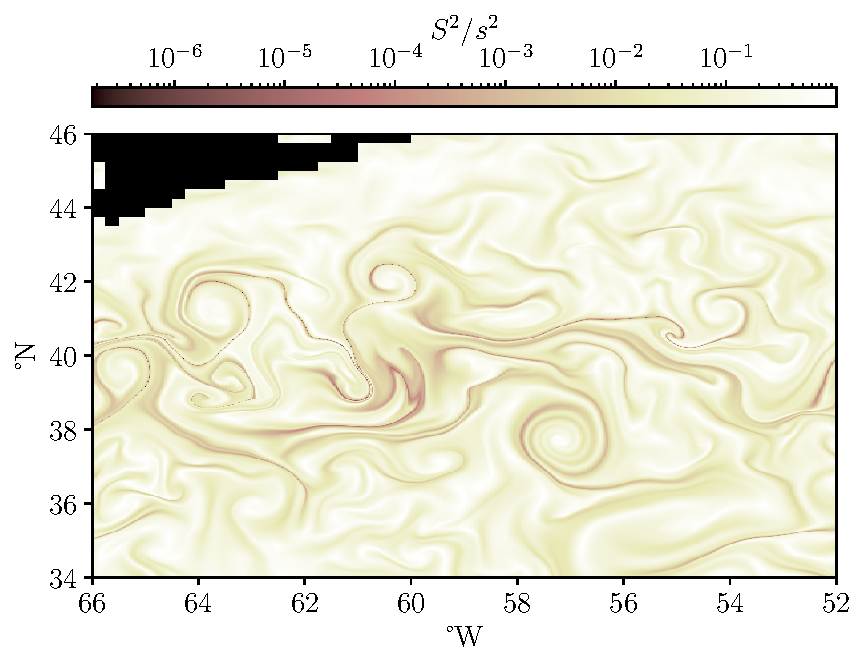
\includegraphics[width=\textwidth]{chp06_applications/figures/gulf_stream/ratio_field_high}
% 		% 	\caption{The ratio of the stochastic sensitivity value (maximum eigenvalue) and the minimum eigenvalue of the covariance matrix, which captures the `narrowness' of the linearised distribution.}
% 		% \end{subfigure}
% 		% \begin{subfigure}[t]{0.49\textwidth}
% 		% 	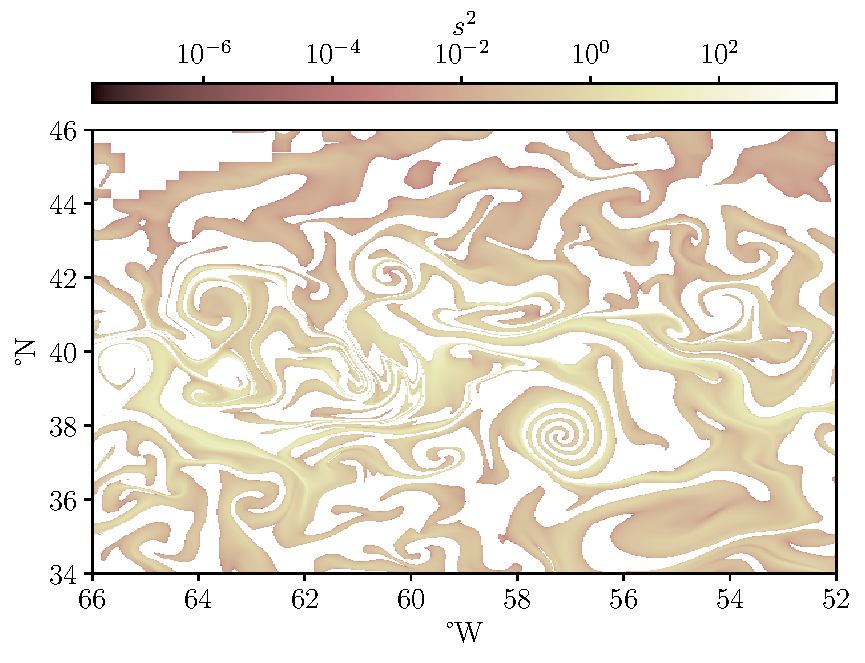
\includegraphics[width=\textwidth]{chp06_applications/figures/gulf_stream/cov_field_high}
% 		% 	\caption{The \((1,2)\)th entry of the covariance matrix, corresponding to the covariance between coordinates.
% 		% 		White indicates regions in which the entry is zero.}
% 		% \end{subfigure}
% 		\caption{Fields computed from the linearisation covariance matrix on a grid of initial conditions, in the same arrangement as \Cref{fig:na_s2} but at a higher resolution of \(0.025^\circ \times 0.025^\circ\).
% 			Note that values near the boundaries of the data and the land are not trustworthy, as the Gaussian approximations do not account for these boundaries.}
% 		\label{fig:na_s2_high}
% 	\end{center}
% \end{figure}

\subsection{The mixture model}
To conclude this example, we will explore a simple implementation of the mixture model algorithm described in \Cref{ch:gmm} to predict the distribution of stochastic solutions about the single trajectory in the previous example.
Again, our aim is to not investigate the algorithm and model in detail, but to rather demonstrate the potential of this algorithm in efficiently approximating the stochastic solution, and therefore as a tool for improving predictions.

As discussed in \Cref{ch:gmm}, we expect that the mixture model approach will work best in moderate noise models and over reasonably short timeframes.
We take the same fixed initial condition \(x_0 = \left(-60.5, 39\right)^{\T}\) but instead consider the position of the drifter at \(t = 3\), so at midnight \DTMdisplaydate{2021}{01}{04}{-1}.
The distribution of numerical samples at this time is given in \Cref{fig:natl_em_3}; the aim here is to use the mixture model algorithm to approximate this non-Gaussian distribution with a small number of Gaussian components, each constructed as solutions to the linearised SDE.
To better understand the impact of the deterministic flow dynamics on the behaviour of the stochastic solution, \Cref{fig:na_hist_t3} plots the evolution of the stochastic samples over three days up to \(t = 3\) and includes contours of the sea surface height at each time.
The contours correspond to the instantaneous streamlines of the deterministic flow.
A majority of the stochastic realisations are propagated by the stream itself, but we see that a number of trajectories leave the stream early and move westwards, creating an arc-like structure of lower density in the empirical distribution.
This behaviour is likely due to the formation and breaking off of an eddy from the stream in the region which the trajectories pass through.
Turning our attention to the distribution of samples at \(t = 3\), the two marginal distributions (in the longitudinal and latitudinal directions) in \Cref{fig:natl_em_3} demonstrate the qualitative departures from Gaussianity mentioned previously: in the longitudinal direction, the distribution of samples is bimodal, whereas in the latitudinal direction we see skew in the southern direction.
The distribution is 2-dimensional, however, so there are aspects of the joint density that are not reflected by the two marginal distributions, such as the curved structure of the density function.
This is a highly non-Gaussian distribution with features such as the scatter of points in the westwards direction that we would like to capture with a mixture model approximation.

\begin{figure}
	\centering
	\begin{subfigure}{0.49\textwidth}
		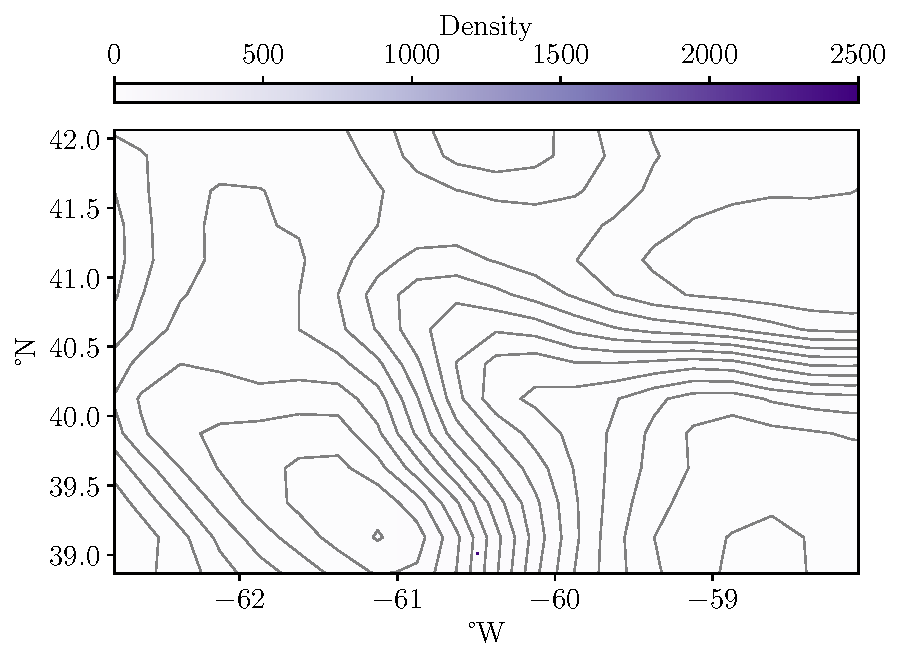
\includegraphics[width=\textwidth]{chp06_applications/figures/gulf_stream/rels_ssh_0.0}
		\caption{Midnight \DTMdisplaydate{2021}{01}{01}{-1} (\(t = 0\)).}
		\label{fig:na_hist_t3_0}
	\end{subfigure}
	\begin{subfigure}{0.49\textwidth}
		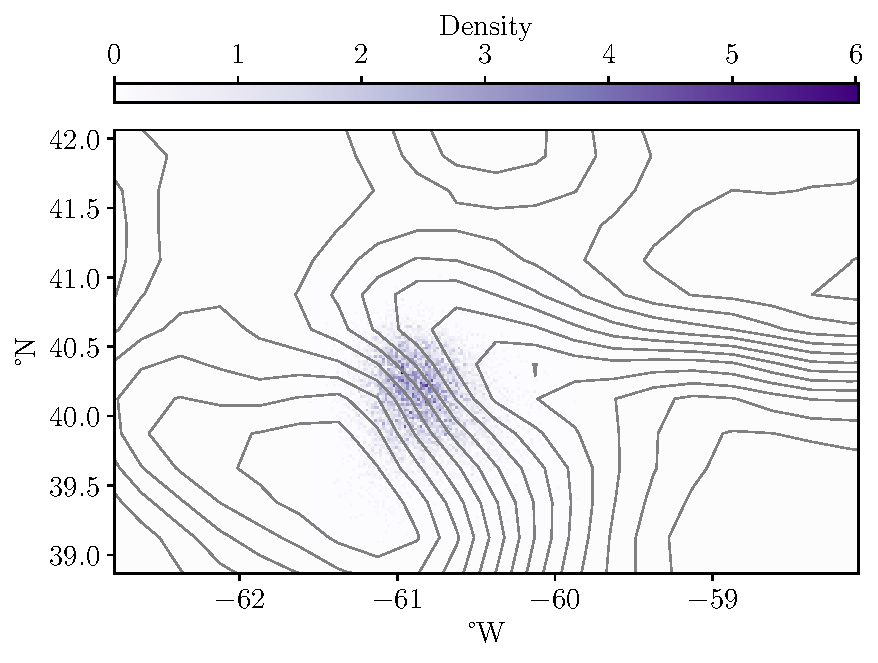
\includegraphics[width=\textwidth]{chp06_applications/figures/gulf_stream/rels_ssh_1.0}
		\caption{Midnight \DTMdisplaydate{2021}{01}{02}{-1} (\(t = 1\)).}
		\label{fig:na_hist_t3_1}
	\end{subfigure}
	\begin{subfigure}{0.49\textwidth}
		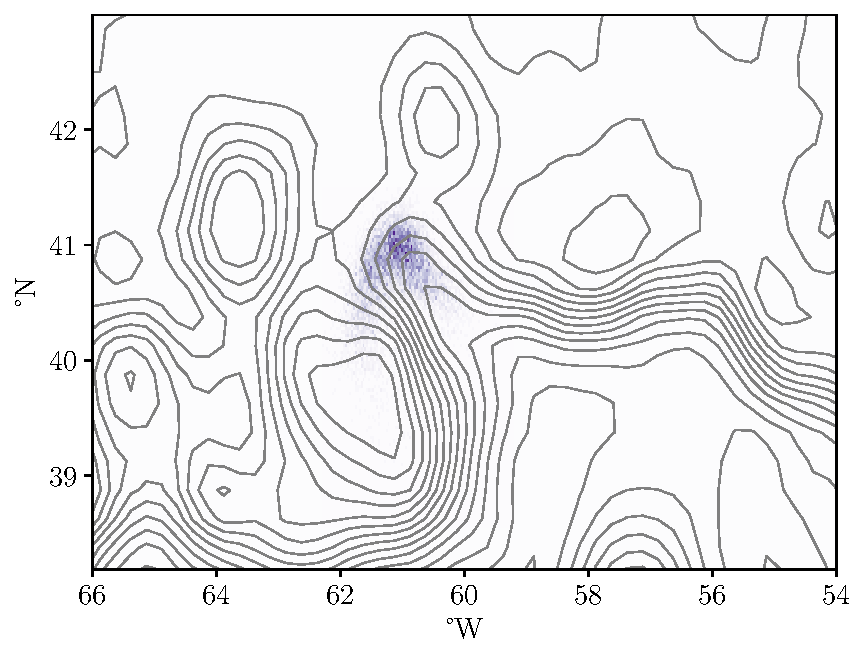
\includegraphics[width=\textwidth]{chp06_applications/figures/gulf_stream/rels_ssh_2.0}
		\caption{Midnight \DTMdisplaydate{2021}{01}{03}{-1} (\(t = 2\)).}
		\label{fig:na_hist_t3_2}
	\end{subfigure}
	\begin{subfigure}{0.49\textwidth}
		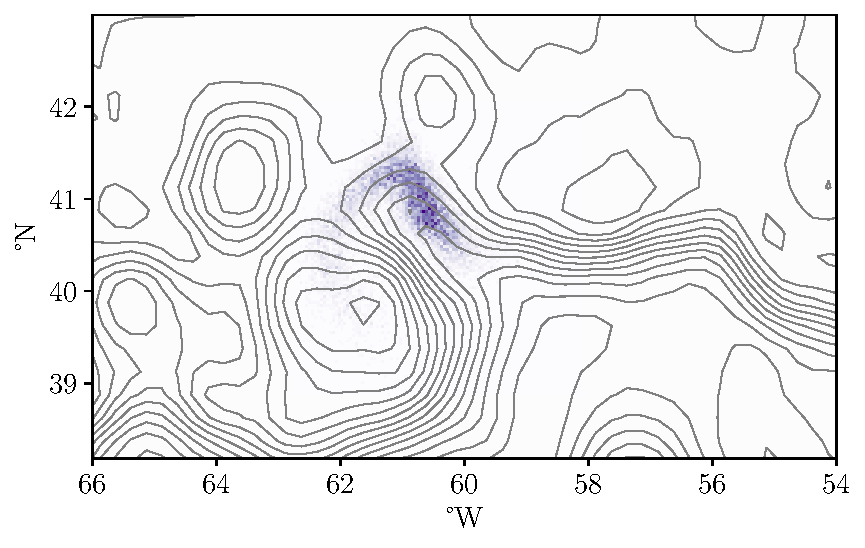
\includegraphics[width=\textwidth]{chp06_applications/figures/gulf_stream/rels_ssh_3.0}
		\caption{Midnight \DTMdisplaydate{2021}{01}{04}{-1} (\(t = 3\)).}
		\label{fig:na_hist_t3_3}
	\end{subfigure}
	\caption{Histograms representing the empirical distribution of the solution to \cref{eqn:natl_sde}, with contours of the sea surface height at each time indicating the flow structure.}
	\label{fig:na_hist_t3}
\end{figure}

First, we shall implement the GMM algorithm with a single manually specified split, which results in a mixture model with 5 components at the final time.
For a given splitting time, we can use the Hellinger distance between the resulting mixture model and the 10000 numerical realisations of the true solution to evaluate the resulting fit.
This allows us to `tune' the choice of splitting time, by finding that which results in the smallest distance.
This method, of course, relies upon us having already obtained the numerical samples over which we are trying to improve computational efficiency.
However, the purposes of this example is to demonstrate that such an optimal time can be found, and to suggest that, once equipped with an appropriate online splitting criterion, the mixture model algorithm provides an efficient ad-hoc method for capturing key features of the distribution.
As a benchmark, the single Gaussian component (shown in \Cref{fig:natl_em_3} overlaid on the histograms of samples) gave a Hellinger distance of approximately 0.48761.

\Cref{fig:na_1split_hell} plots the Hellinger distance for each run of the mixture model algorithm with the split at times \(t_s\), each varying by an hour.
The Hellinger distance between the single Gaussian approximation and the same EM samples is also indicated by the green line.
We can see that an early split time (less than \(t = 2\), say) results in a mixture model that improves over the single Gaussian approximation.
When the split occurs later, the quality of the resulting mixture model worsens.\td{Any way to interpret this? Not getting enough information of the surrounding flow?}
The minimum Hellinger distance of approximately 0.30191 occurs with a split at \(t_s = 33/24\) days, or at 9am \DTMdisplaydate{2021}{01}{02}{-1}, which we take as our `best' fit.
We compare the resulting mixture model against the numerical samples in \Cref{fig:na_1split_best}, in the same fashion as \Cref{fig:natl_em} where contours of the mixture probability density function are shown on the joint histogram and the marginal PDFs on each marginal histogram.
However, the mixture fails to capture the spread of samples in the southern direction, even though this only corresponds to a small proportion of the samples.


\begin{figure}
	\begin{center}
		\begin{subfigure}{\textwidth}
			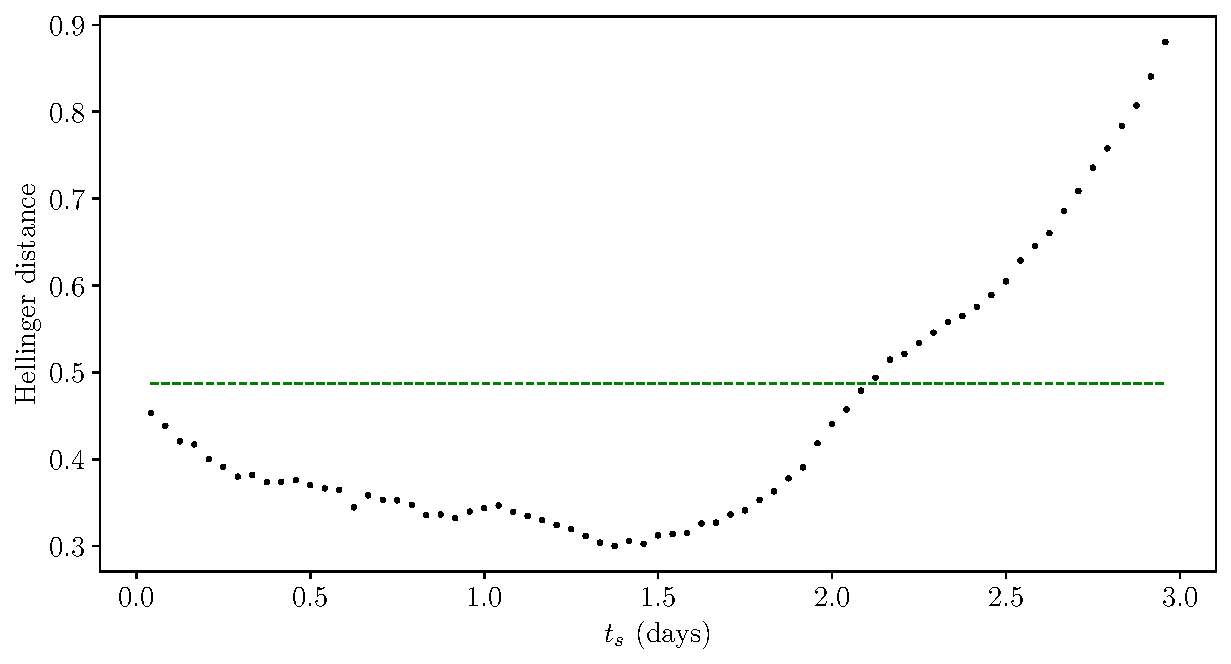
\includegraphics[width=\textwidth]{chp06_applications/figures/gulf_stream/hell_dist_split}
			\caption{The Hellinger distance between stochastic samples and the mixture model implemented with a single split at time \(t_s\).}
			\label{fig:na_1split_hell}
		\end{subfigure}
		\begin{subfigure}{\textwidth}
			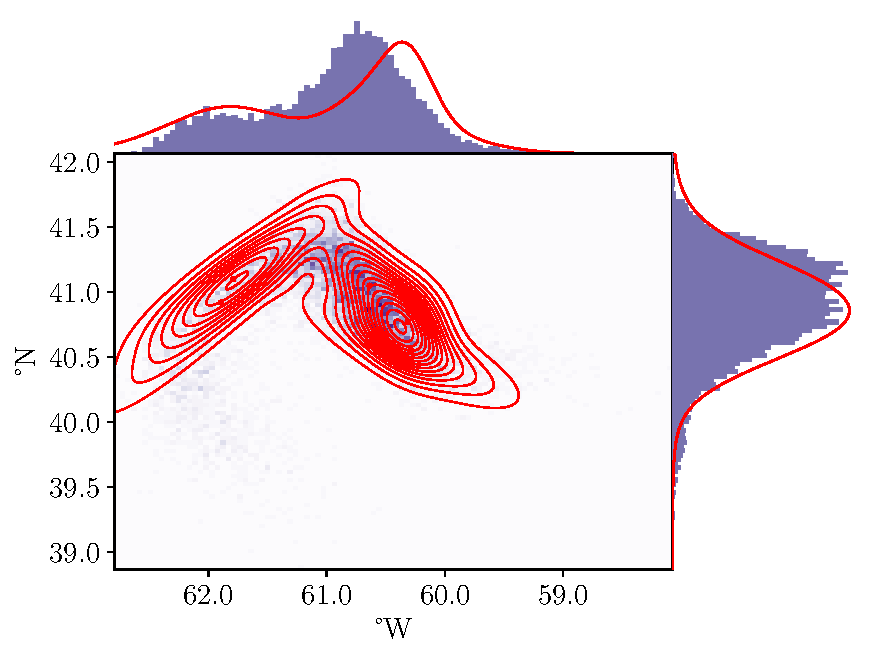
\includegraphics[width=\textwidth]{chp06_applications/figures/gulf_stream/gmm_split_best}
			\caption{The best-fitting mixture model, with a single split at \(t_s = \) ().
				The joint histogram (center) includes the component means (as red points) and continues of the mixture density.
				Each axis provides marginal histograms of the numerical samples, with the corresponding marginal PDFs of the mixture density in red.}
			\label{fig:na_1split_best}
		\end{subfigure}
		\caption{The Gaussian mixture model algorithm implemented with a single on the Gulf Stream trajectory with initial condition \(x_0 = \left(-60.5, 39\right)^{\T}\) and over the timespan from midnight \DTMdisplaydate{2021}{01}{01}{-1} to midnight \DTMdisplaydate{2021}{01}{04}{-1}.}
		\label{fig:na_1split}
	\end{center}
\end{figure}


The optimal configuration with two splits has the first at \(t_{s,1} = 3/4\) (at 6pm \DTMdisplaydate{2021}{01}{01}{-1}) and the second at \(t_{s,2} = 43/24\) (at 7pm \DTMdisplaydate{2021}{01}{02}{-1}), and results in a Hellinger distance of approximately 0.14684.
This distance is a substantial improvement over both the single Gaussian component and the mixture model with a single split.
In \Cref{fig:na_2split_best}, we compare this mixture density against the stochastic samples, in the same arrangement as \Cref{fig:na_1split_best}.

\begin{figure}
	\begin{center}
		\begin{subfigure}{\textwidth}
			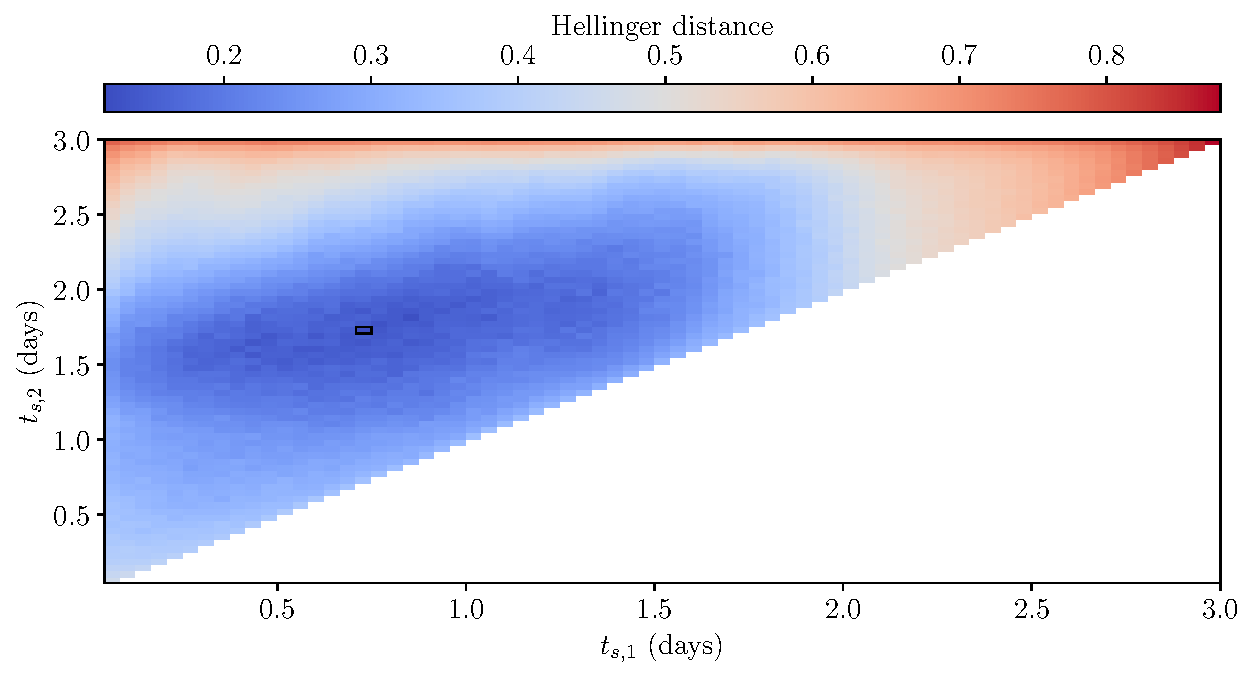
\includegraphics[width=\textwidth]{chp06_applications/figures/gulf_stream/hell_dist_2split}
			\caption{Two splits: the first at \(t_{s,1}\) days, and the second at \(t_{s,2} > t_{s,1}\) days.
				When \(t_{s,1} = t_{s,2}\), the result for a single split at that time is shown for comparison.
				The minimising value is indicated by the black box.}
			\label{fig:na_2split_hell}
		\end{subfigure}
		\begin{subfigure}{\textwidth}
			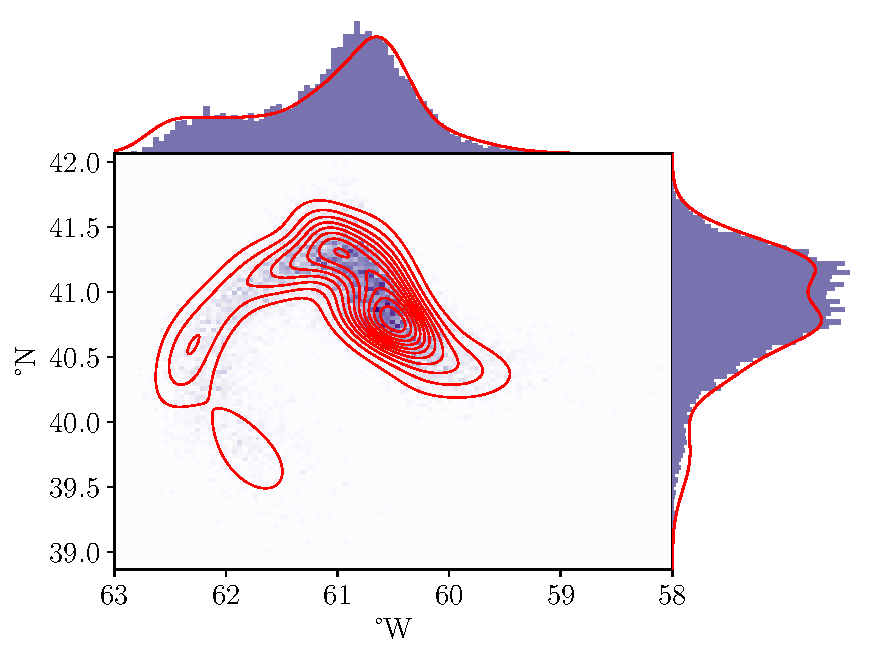
\includegraphics[width=\textwidth]{chp06_applications/figures/gulf_stream/gmm_2split_best}
			\caption{The best-fitting mixture model (according to the Hellinger distance) with two splits on each component.}
			\label{fig:na_2split_best}
		\end{subfigure}
		\caption{}
		\label{fig:na_2split}
	\end{center}
\end{figure}


With a simple implementation of the mixture model, we are able to capture key features and provide a close approximation of the distribution of the solution at \(t = 3\).
Estimating this distribution is a difficult problem, as the deterministic dynamics are complicated and highly non-linear, and the non-uniformity of error in the observations used to construct it means that the noise is multiplicative.

Evaluating the mixture model and finding the best splitting times required a set of numerical realisations of the SDE solution, when our aim is to avoid this computational cost.
However, we continue to emphasise that this example is demonstrative and the mixture model has only been proposed as an outline of an algorithm, and at this point is highly ad-hoc.
Nonetheless, the results of this section are encouraging.
There are clear splitting times in \Cref{fig:na_1split,fig:na_2split} for which the mixture model results in an optimal (with respect to the Hellinger distance) fit.\td{Need to articulate this better.}
Once equipped with an appropriate splitting criterion, the mixture model algorithm could become a highly effective method for circumventing bulk simulation in stochastic systems.
Even in lieu of this splitting criterion, the mixture model provides an explicit form for the probability density function, which may lend itself to further applications.
We discuss this in detail in \Cref{sec:gmm_extensions}.



% \section{Empirical model of sea-surface winds}
% \td{Possibly something funky to try - use the observed data to construct the FLOW MAP, and then compute based purely on that!! The paper by \cite{Sura_2003_StochasticAnalysisSouthern} basically interpolates the data then uses finite differences and statistical averaging to find the ODE. But we can avoid that step entirely by just treating the data!}

% Empirical, or data-driven, stochastic models are used heavily in climate science, where components of the model are derived by fitting to time series of observed data.
% In this section, we follow the method of \citet{EggerJonsson_2002_DynamicModelsIcelandic} and \citet{Sura_2003_StochasticAnalysisSouthern} to construct from observed data a stochastic differential equation model for the time evolution of sea surface wind velocities.

% Consider an \(n\)-dimensional state variable \(x_t\) governed by the It\^o SDE
% \begin{equation}\label{eqn:sde_emp}
% 	\dif x_t = A(x_t) + B(x_t)\dif W_t,
% \end{equation}
% where \(W_t\) is an \(n\)-dimensional Wiener process and the coefficients \(A \colon \R^n \to \R^n\) and \(B \colon \R^n \to \R^{n\times n}\) are permitted to vary with state but not time.
% To determine the drift and diffusion directly from observed data, we consider the statistical definitions of the coefficients:
% \begin{subequations}\label{eqn:sde_coef_stat}
% 	\begin{align}
% 		A(x)          & = \lim_{\delta t \to 0}\frac{1}{\delta t}\avg{x_{t + \delta t} - x} \label{eqn:sde_coef_stat_drift}                                                \\
% 		B(x)B(x)^{\T} & = \lim_{\delta t \to 0}\frac{1}{\delta t}\avg{\left(x_{t + \delta} - x\right)\left(x_{t + \delta} - x\right)^{\T}}, \label{eqn:sde_coef_stat_diff}
% 	\end{align}
% \end{subequations}
% where the expected values are taken over all trajectories solving \cref{eqn:sde_emp} with \(x_{t} = x\).
% The expressions in \cref{eqn:sde_coef_stat} arise by considering the Fokker-Planck equation corresponding to \eqref{eqn:sde_emp} \citehere.

% Now suppose that we have a collection of \(K\) time series, each corresponding to a solution trajectory of \cref{eqn:sde_emp} and evaluated at (possibly non-uniform) times \(t_0, t_1, \dotsc, t_n\).
% Let the \(k\)th time series be denoted by
% \[
% 	\set{X_{0}^{(k)}, X_{1}^{(k)}, \dotsc, X_{n}^{(k)}}.
% \]
% The definitions in \cref{eqn:sde_coef_stat} are only correct in the limit as \(\delta t\) approaches zero, which we cannot obtain from our discrete-time data, and involves expectations of the theoretical solution to \eqref{eqn:sde_emp}.
% However, we can approximate the expressions using a finite difference for the limit and binned sample estimates for the expectations.




\section{Epidemiology}



Stochastic differential equations emerge from these discrete models in the limit of an infinite population size.
Analogous to the behaviour of nonlinear stochastic differential equations in small noise limits (as established by \citet{FreidlinWentzell_1998_RandomPerturbationsDynamical} and our work in \Cref{ch:linear_theory}), the density process converges to the solution to a system of ordinary differential equations (known as the \emph{fluid limit} in some literature).
Moreover, the stochastic variation of the process about this deterministic limit converges to the solution to a linear stochastic differential equation (known as the \emph{diffusion limit}).
We summarise these results in \Cref{sec:epi_limits}.




\subsection{A very brief overview of population processes}
A common model for population process are continuous-time Markov chains (CTMCs)
Here, we provide only a brief overview of population processes; for a more detailed intorduction, see \citehere.

The population process is described by the transition function \(q\colon \mathcal{S}\times\mathcal{S} \to [0,\infty)\), where \(q(x,y)\) describes the rate at which

A single sample \(X\) from the population process at time \(T\) can be simulated with the following procedure \citep{Gillespie_1977_ExactStochasticSimulation}:
\begin{enumerate}
	\item Initialise \(X = X_0\), the initial state of the process.
	      If the initial state is uncertain, sample \(X\) from the initial state distribution.

	\item Sample the time \(\tau\) to the next event as
	      \[
		      \tau \isExp{\sum_{\substack{l \in \R^n \\ l \neq 0,\, y + l \in \mathcal{S}}}{q\!\left(X, X + l\right)}},
	      \]
	      and set \(t = t + \tau\).

	\item If \(t > T\), terminate.
	      Otherwise, sample the next state from the set of possible transitions \(\setc{l \in \R^n}{l \neq 0,\, y + l \in \mathcal{S}}\), where the probability of transitioning from \(X\) to \(X + l\) is given by
	      \[
		      \frac{q\!\left(X, X + l\right)}{\sum_{\substack{k \in \R^n \\ k \neq 0,\, y + k \in \mathcal{S}}}{q\!\left(X, X + k\right)}}.
	      \]
	      Set \(X\) to this state.

	\item Repeat Steps 2 and 3 until the sample path is terminated.

\end{enumerate}
The result is a single sample \(X\) of the population process at time \(T\).
The sum is taken across all the possible transitions from the current state.
Note that typically most of these rates are zero, so the sum does not need to be taken over the entire state space.

\subsection{Large population diffusion limits}\label{sec:epi_limits}
In the limit of large population sizes, a deterministic ordinary differential equation and linear stochastic differential equation arise from certain population processes, despite these processes being discrete.
A population process is \emph{density dependent} (in the sense of \citet{Kurtz_1970_SolutionsOrdinaryDifferential}) if there is a parameter \(N\) such that
\begin{equation}
	q\!\left(n, n+l\right) = Nf\!\left(\frac{n}{N}, l\right),
	\label{eqn:ctmc_dens_dep}
\end{equation}
where \(f\) is a suitable function and \(n, n+l \in \mathcal{S}\).
Typically, \(N\) is related to the size of the system and \(n / N\) is a population density.
The condition in \cref{eqn:ctmc_dens_dep} states that the transition rates of the process \(X_t\) depends on \(X_t\) itself only through the density \(X_t / N\).

Let \(Y_t^{(N)}\) describe the \(n\)-dimensional density process, i.e. with \(i\)th element \(X_t^{(i)} / N\).
Theorem 3.1 of \citet{Kurtz_1970_SolutionsOrdinaryDifferential} establishes that in the large population limit \(N \to \infty\), the density process \(Y_t^{(N)}\) converges in probability to a deterministic trajectory \(Y_t^{(\infty)}\) solving the ODE
\begin{equation}
	\dod{Y_t^{(\infty)}}{t} = Q\!\left(Y_t^{(\infty)}\right), \quad Y_0^{(\infty)} = X_0 / N,
	\label{eqn:ctmc_dens_dep_ode}
\end{equation}
where
\[
	Q\!\left(y\right) = \sum_{\substack{l \in \R^n \\ l \neq 0,\, y + l \in \mathcal{S}}}{l f\!\left(y, l\right)}.
\]
For large \(N\), the density process has small variation and is ``close'' to the deterministic solution to \cref{eqn:ctmc_dens_dep_ode}.
This result is analogous to that for small noise SDEs; the solution to a stochastic differential equation formally converges to that of a deterministic system (involving only the drift term) in the limit of small noise, which is a result established by large deviations principles \citep[e.g]{FreidlinWentzell_1998_RandomPerturbationsDynamical}.

\citet{Kurtz_1971_LimitTheoremsSequences} then established a stronger result, showing that the variation of the density process about this deterministic limit is captured by an It\^o diffusion.
Define the scaled process
\[
	Z_t^{(N)} = \sqrt{N}\left(Y_t^{(N)} - Y_{t}^{(\infty)}\right),
\]
then Theorem 3.5 of \citet{Kurtz_1971_LimitTheoremsSequences} proves that \(Z_t^{(N)}\) converges in distribution (weakly) to an It\^o diffusion \(Z_t^{(\infty)}\) solving
\begin{equation}
	\dif Z_t^{(\infty)} = \nabla Q\!\left(Y_t^{(\infty)}\right) Z_t^{(\infty)}\dif t + G\!\left(Y_t^{(\infty)}\right)\dif W_t, \quad Z_0^{(\infty)} = 0,
	\label{eqn:ctmc_dens_dep_sde}
\end{equation}
where \(W_t\) is an \(n\)-dimensional Wiener process and the \(n \times n\) diffusion matrix \(G\) is such that
\begin{equation}
	\left[G\!\left(y\right)G\!\left(y\right)^{\T}\right]_{ij} = \sum_{\substack{l \in \R^n \\ l \neq 0,\, y + l \in \mathcal{S}}}{l_i l_j f\!\left(y,l\right)}
	\label{eqn:ctmc_dens_dep_sde_diff_cond}
\end{equation}
Any choice of diffusion matrix \(G\) such that \cref{eqn:ctmc_dens_dep_sde_diff_cond} is satisfied will result in a statistically identical diffusion process \(Z_0^{(\infty)}\).

The limiting SDE \cref{eqn:ctmc_dens_dep_sde} is equivalent to the unscaled SDE
\begin{equation}
	\dif L_t^{(N)} = \left[Q\!\left(Y_t^{(\infty)}\right) + \frac{1}{\sqrt{N}} \nabla Q\!\left(Y_t^{(\infty)}\right)\left(L_t^{(N)} - Y_t^{(\infty)}\right)\right]\dif t + \frac{1}{\sqrt{N}}G\!\left(Y_t^{(\infty)}\right)\dif W_t,
	\label{eqn:ctmc_sde_lin_lim}
\end{equation}
which is a linearisation of the nonlinear SDE
\begin{equation}
	\dif \hat{Y}^{(N)}_t = Q\!\left(\hat{Y}^{(N)}_t\right)\dif t + \frac{1}{\sqrt{N}}G\!\left(\hat{Y}_t^{(N)}\right)\dif W_t
	\label{eqn:ctmc_sde_lim_nonlin}
\end{equation}
about the deterministic limit \(Y_t^{(\infty)}\).
There is intuition behind the choices of drift and diffusion in \cref{eqn:ctmc_sde_lim_nonlin}.
For sufficiently large \(N\), the drift term \(Q\) captures the average (macroscopic) behaviour of the density process.
The diffusion term captures the microscopic behaviour resulting from individual transition events, and the uncertainty in this is parameterised with the Wiener process \(W_t\).




\td{Explain how this is analogous to the proceeding work}
However, a key difference is that in the SDE linearisation procedure, we start from a continuous state-space process and arrive at a continuous state-space process in the limit.
Whereas, in the CTMC diffusion limit, the converging process is on a \emph{discrete} state-space and the limit is on a continuous one.




Thus, we expect that the mixture model algorithm we have described may find a place in moderate-population compartmental models, where the population is large enough to be ``reasonably'' approximated by the continuum and SDE equations, but small enough to exhibit non-Gaussian behaviour.
Regardless, our error bound derived in \Cref{ch:linear_theory} still has a place in this literature.



\subsection{Example 1: the SIR model}
Assume a fixed population of \(N\) individuals, each classified into one of three compartments: susceptible (\(S\)) and infected (\(I\)), and recovered/removed (\(R\)).
At any time, the number of removed individuals can be computed as \(R = N - S - I\), so we only need to specify a two-dimensional model for the number of susceptible and infected individuals.
Such a process can model the spread of a disease in a homogeneously mixing population in which susceptible individuals become infected upon contact with infected individuals, and once infected individuals recover they are no longer infectious or susceptible to reinfection.
The state space is then
\[
	\mathcal{S} = \setc{\left(s,i\right)}{s,i \in \set{0,1,\dotsc,N}, \, s + i \leq N},
\]
where the number of recovered individuals at any time is \(N - S - I\).
The events and the corresponding transition probabilities are described in \Cref{fig:sir_transition}.

\usetikzlibrary{automata,positioning,arrows}
\tikzset{->, node distance = 2cm}
\begin{figure}
	\begin{center}
		\begin{tabular}{|c|c|c|c|}
			\hline
			Transition & \multicolumn{2}{c|}{Event} & Rate \(\lambda_i\)                                                    \\ \hline
			1          & Infection                  & \(\left(S, I\right) \to \left(S-1, I + 1\right)\) & \(\beta S I / N\) \\ \hline
			2          & Recovery                   & \(\left(S,I\right) \to \left(S, I - 1\right)\)    & \(\gamma I\)      \\ \hline
		\end{tabular} \\
		\begin{tikzpicture}
			\node[state] (S) {\(S\)};
			\node[state, right of = S] (I) {\(I\)};
			\node[state, right of = I] (R) {\(R\)};
			\draw (S) edge[above] node{(1)} (I)
			(I) edge[above] node{(2)} (R);
		\end{tikzpicture}
		\caption{Transition probabilities of the SIR compartmental model.}
		\label{fig:sir_transition}
	\end{center}
\end{figure}
The population process is density dependent, with
\[
	f\left((s,i), l\right) = \begin{cases}
		\beta s i, & \text{if } l = \left(-1, 1\right), \\
		\gamma i,  & \text{if } l = \left(0,-1\right)   \\
		0,         & \text{otherwise}.
	\end{cases}
\]
Let \(X_t^{(N)} = \left(S_t / N, I_t / N\right)\) denote the proportion of susceptible and infected individuals and at time \(t\).
The corresponding deterministic differential equation approximation is
\[
	\dod{X_t^{(\infty)}}{t} = \begin{bmatrix}
		-\beta X_t^{(\infty,1)} X_t^{(\infty, 2)} \\
		\beta X_t^{(\infty,1)} X_t^{(\infty, 2)} -\gamma X_t^{(\infty, 2)}
	\end{bmatrix},
\]
where \(X_t^{(\infty)} \equiv \left(X_t^{(\infty, 1)}, X_t^{(\infty, 2)}\right)^{\T}\).
Consider the scaling
\[
	Z_t^{(N)} = \sqrt{N}\left(X_t^{(N)} - X_t^{(\infty)}\right),
\]
then \citet{Kurtz_1971_LimitTheoremsSequences} establish that in the limit \(N \to \infty\), the scaled process \(Z_t^{(N)}\) will converge in distribution to the It\^o diffusion \(Z_t^{(\infty)}\) solving
\begin{equation}
	\dif Z_t^{(\infty)} = \begin{bmatrix}
		-\beta X_t^{(\infty, 2)} & -\beta X_t^{(\infty, 1)}         \\
		\beta X_t^{(\infty, 2)}  & \beta X_t^{(\infty, 1)} - \gamma
	\end{bmatrix} Z_t^{(\infty)}\dif t + g\!\left(X_t^{(\infty)}\right)\dif W_t
	\label{eqn:sir_diff_limit}
\end{equation}
where the diffusion matrix \(G\) satisfies
\[
	g\!\left(X_t^{(\infty)}\right)g\!\left(X_t^{(\infty)}\right)^{\T} = \begin{bmatrix}
		\beta X_t^{(\infty, 1)} X_t^{(\infty, 2)}  & -\beta X_t^{(\infty, 1)} X_t^{(\infty, 2)}                              \\
		-\beta X_t^{(\infty, 1)} X_t^{(\infty, 2)} & \beta X_t^{(\infty, 1)} X_t^{(\infty, 2)} + \gamma X_{t}^{(\infty, 2)}.
	\end{bmatrix}
\]
Any choice of \(g\) satisfying this property will result in a statistically identical diffusion process, so we take
\[
	g\!\left(X_t^{(\infty)}\right) = \begin{bmatrix}
		\sqrt{\beta X_t^{(\infty, 1)} X_t^{(\infty, 2)}}  & 0                               \\
		-\sqrt{\beta X_t^{(\infty, 1)} X_t^{(\infty, 2)}} & \sqrt{\gamma X_t^{(\infty, 2)}}
	\end{bmatrix}.
\]
The stochastic differential equation \cref{eqn:sir_diff_limit} is a linear in the same form as the linearisation \cref{eqn:linear_sde} considered in \Cref{ch:linear_theory}, and so is solved by the Gaussian process
\[
	Z_t^{(\infty)} \isGauss{0,\, \Sigma_0^t\!\left(X_0^{(\infty)}\right)},
\]
where \(\Sigma_0^t\!\left(X_0^{(\infty)}\right)\) is the symmetric positive-definite solution to the matrix differential equation
\[
	\dod{\Sigma_0^t\!\left(X_0^{(\infty)}\right)}{t} = \begin{multlined}[t]
		\begin{bmatrix}
			-\beta X_t^{(\infty, 2)} & -\beta X_t^{(\infty, 1)}         \\
			\beta X_t^{(\infty, 2)}  & \beta X_t^{(\infty, 1)} - \gamma
		\end{bmatrix}\Sigma_0^t\!\left(X_0^{(\infty)}\right) \\
		+ \Sigma_0^t\!\left(X_0^{(\infty)}\right)\begin{bmatrix}
			-\beta X_t^{(\infty, 2)} & \beta X_t^{(\infty, 1)}          \\
			-\beta X_t^{(\infty, 2)} & \beta X_t^{(\infty, 1)} - \gamma
		\end{bmatrix} \\
		+ \begin{bmatrix}
			\beta X_t^{(\infty, 1)} X_t^{(\infty, 2)}  & -\beta X_t^{(\infty, 1)} X_t^{(\infty, 2)}                              \\
			-\beta X_t^{(\infty, 1)} X_t^{(\infty, 2)} & \beta X_t^{(\infty, 1)} X_t^{(\infty, 2)} + \gamma X_{t}^{(\infty, 2)}.
		\end{bmatrix}.
	\end{multlined}
\]

For the purposes of this demonstrative example, take the rate of infection to be \(\beta = 1.2\) and the rate of recovery to be \(\gamma = 0.8\).
These values correspond to a reproductive number of \(R_0 = 1.5\), meaning that in the early stage of the population process, a single infected individual results in an average of 1.5 new infections.

We first show that stochastic simulations of the density process for the SIR model converge to the Gaussian process solving \cref{eqn:sir_diff_limit}, in a similar manner to how we validated our convergence results for stochastic differential equations in \Cref{ch:linear_numerics}.
For several different population sizes, we generate \(100000\) Monte-Carlo realisations of the CTMC SIR process at time \(t = 5\) and plot histograms of the corresponding density processes in \Cref{fig:sir_gauss_rels}.
Each population process is initialised with 10\% of the \(M\) individuals infected and the remaining 90\% susceptible.
For large populations (\(M = 1000\) and \(M = 10000\)), the diffusion limit appears to provide a reasonable approximation for the density process, as expected from the theory of \citet{Kurtz_1970_SolutionsOrdinaryDifferential,Kurtz_1971_LimitTheoremsSequences}.
We therefore also expect that our developments using the Gaussian process solution to a linearised SDE can be applied in these situations.
\td{Fix alignments in histograms.}

\begin{figure}
	\begin{center}
		\begin{subfigure}{0.49\textwidth}
			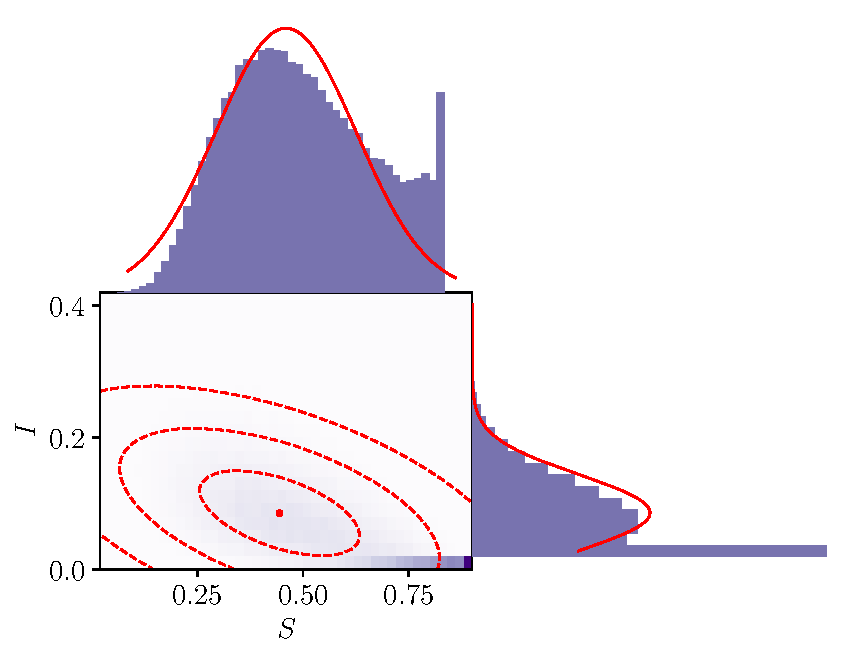
\includegraphics[width=\textwidth]{chp06_applications/figures/sir/sir_pairwise_50}
			\caption{\(M = 50\)}
			\label{fig:sir_gauss_rels_1}
		\end{subfigure}
		\begin{subfigure}{0.49\textwidth}
			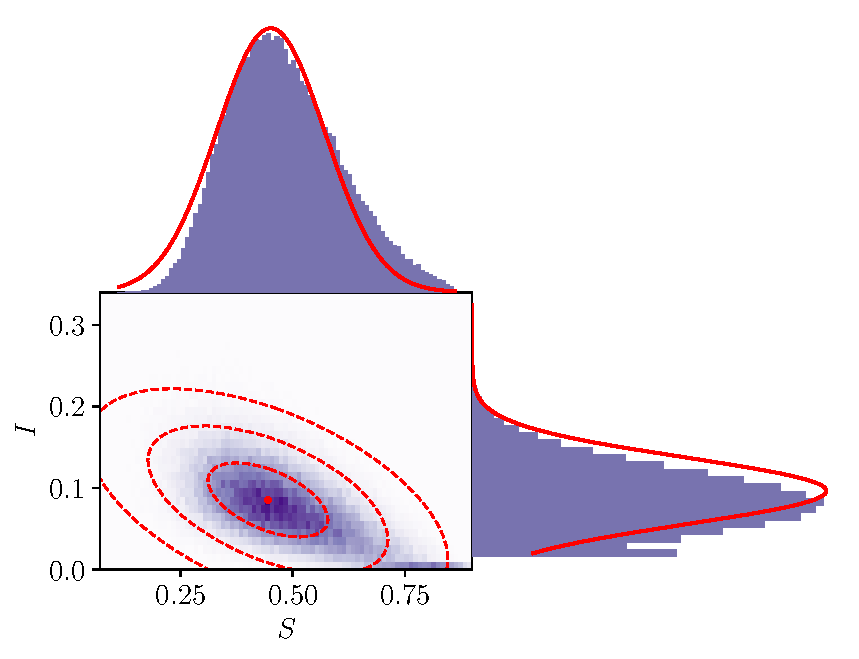
\includegraphics[width=\textwidth]{chp06_applications/figures/sir/sir_pairwise_100}
			\caption{\(M = 100\)}
			\label{fig:sir_gauss_rels_2}
		\end{subfigure}
		\begin{subfigure}{0.49\textwidth}
			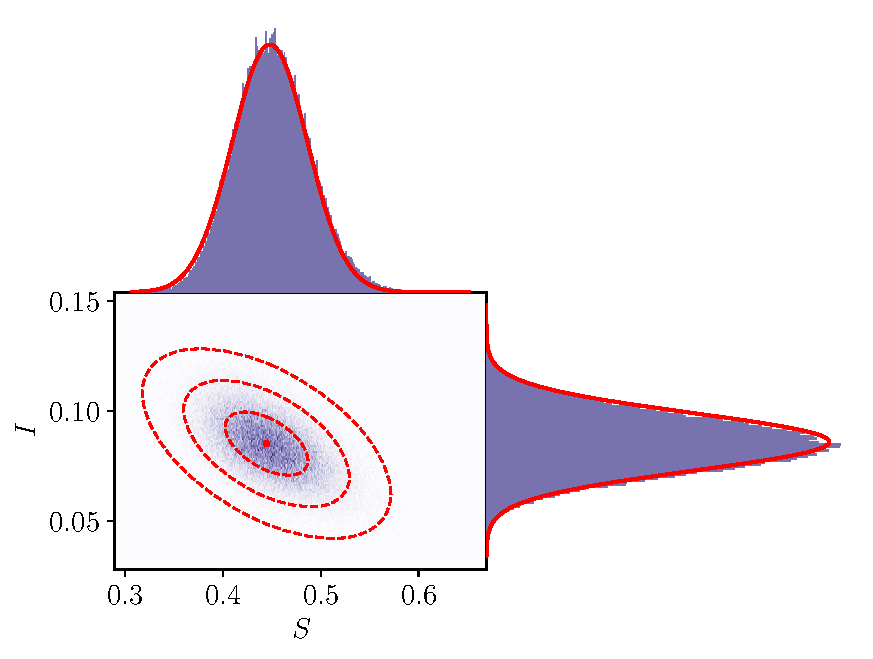
\includegraphics[width=\textwidth]{chp06_applications/figures/sir/sir_pairwise_1000}
			\caption{\(M = 1000\)}
			\label{fig:sir_gauss_rels_3}
		\end{subfigure}\begin{subfigure}{0.49\textwidth}
			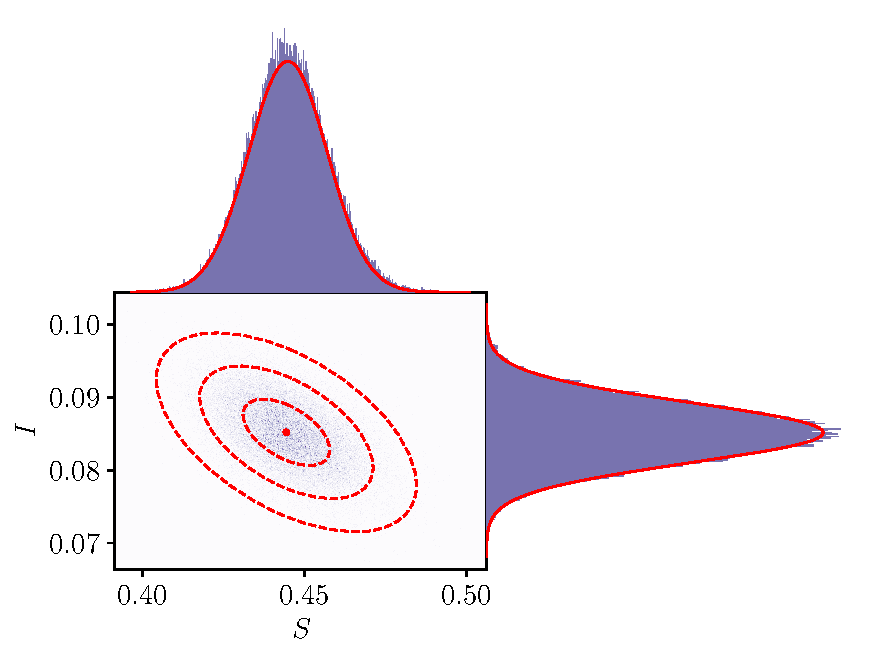
\includegraphics[width=\textwidth]{chp06_applications/figures/sir/sir_pairwise_10000}
			\caption{\(M = 10000\)}
			\label{fig:sir_gauss_rels_4}
		\end{subfigure}
		\caption{Histograms of Monte-Carlo simulations of the density process for the SIR model (with marginal plots on each axis), and the probability density function of the corresponding solution to the diffusion limit \cref{eqn:sir_diff_limit} plotted in red.
			Each sample path is initialised with 10\% of the population infected (i.e. \(x_0 = \left(0.1, 0.9\right)^{\T}\)).}
		\label{fig:sir_gauss_rels}
	\end{center}
\end{figure}

However, \Cref{fig:sir_gauss_rels} also highlights the limitations of using Gaussian approximations for certain types of stochastic processes.
An \(n\)-dimensional Gaussian random variable has support on the entirety of \(\R^n\); that is, for any non-empty subset of \(\R^n\), there is a non-zero probability of the variable taking a value in that set.
However, in many situations we can enforce (often from physical considerations) boundary conditions on the state variable.
In the SIR model, the \(I = 0\) and \(S = 0\) boundaries are \emph{absorbing}, in the sense that once the stochastic process reaches those states, it remains there indefinitely with probability \(1\).
We also saw another example of boundaries in the Gulf Stream example in \Cref{sec:appl_ocean}; the dataset only contained velocity
Boundary issues were avoided by ensuring that the evolution of the deterministic trajectory was sufficiently far from the boundaries and the scale of uncertainty small enough so that the probability of a stochastic trajectory nearing the boundary is negligible.
An absorbing boundary can be accounted for by setting both the drift and diffusivity in the stochastic differential equation to zero on the boundary.
However, such adjustments will often violate the requirements of smoothness in these terms set out in \Cref{hyp:smooth}.
More generally, one can stochastic differential equations with boundary conditions, and it can be shown that such SDEs do in fact have unique solutions; an introduction to the formal treatment of stochastic differential equations with boundary conditions is provided by \citet{Pilipenko_2014_IntroductionStochasticDifferential}.
However, the presence of boundary conditions is beyond the scope of this thesis and we will instead ensure that we choose initial conditions and values so that the impact of boundaries is negligible.


For large populations, the Gaussian diffusion limit is a well-used approximation that has been employed across many different modelling scenarios \citep[e.g.]{PollettEtAl_2010_ModellingPopulationProcesses}.
Rather, we are interested in the moderate-sized population case where the population is large enough to limit the practicality of Monte-Carlo simulation, but is small enough that the density process distributions demonstrate departures from Gaussianity.
Our aim is to employ the GMM algorithm to provide computationally efficient approximations in these scenarios, which we explore on a 5-dimensional example informed by real data in the next section (\Cref{sec:epi_5d}).

Next, we will compute the stochastic sensitivity field on the set of (physically relevant) initial conditions to the SIR model.



\begin{figure}
	\begin{center}
		\begin{subfigure}{0.49\textwidth}
			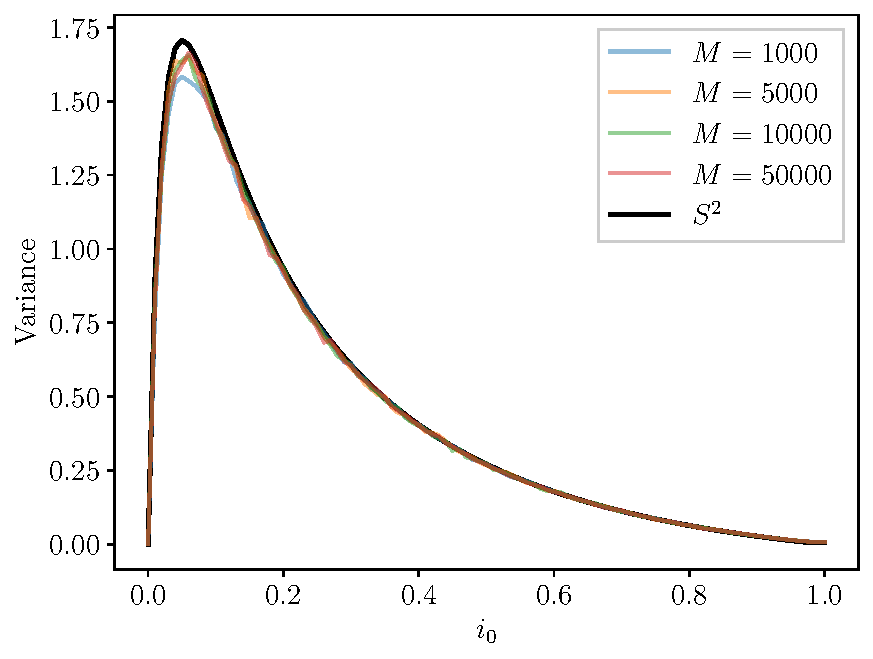
\includegraphics[width=\textwidth]{chp06_applications/figures/sir/sir_s2_1.0_1.0.pdf}
			\caption{\(\beta = 1\), \(\gamma = 1\) (\(R_0 = 1\))}
		\end{subfigure}
		\begin{subfigure}{0.49\textwidth}
			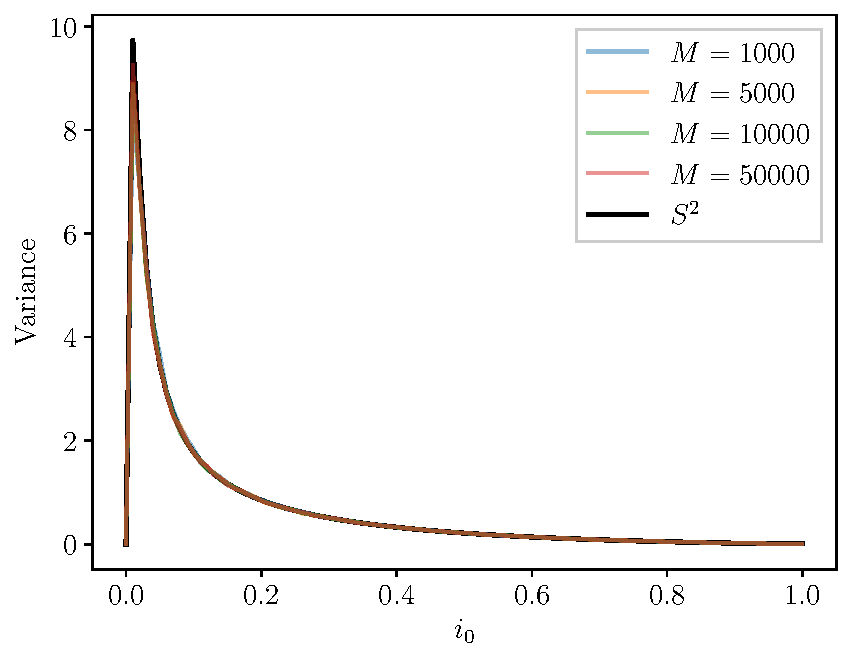
\includegraphics[width=\textwidth]{chp06_applications/figures/sir/sir_s2_1.5_1.0.pdf}
			\caption{\(\beta = 1.5\), \(\gamma = 1\) (\(R_0 = 1.5\))}
		\end{subfigure}\begin{subfigure}{0.49\textwidth}
			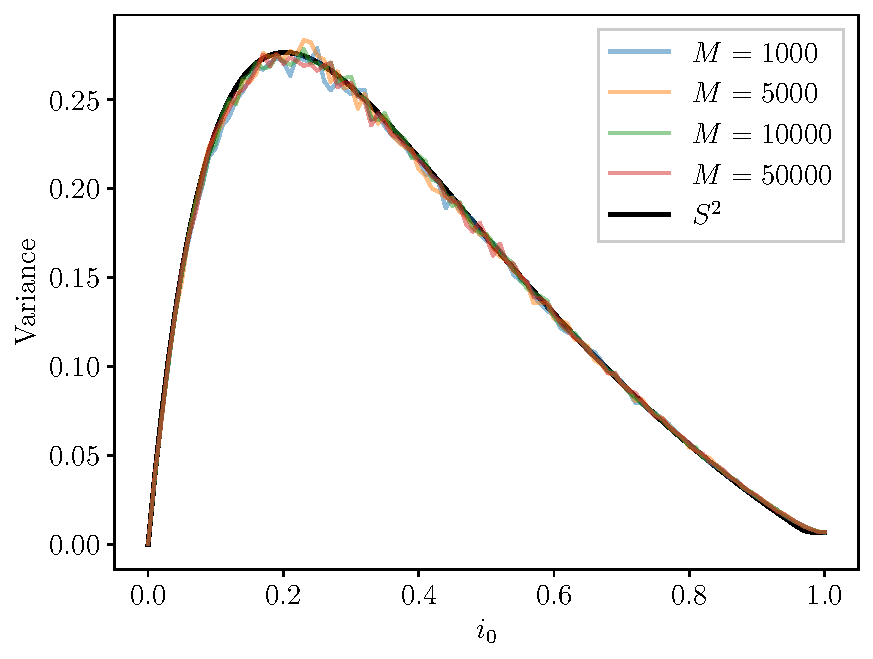
\includegraphics[width=\textwidth]{chp06_applications/figures/sir/sir_s2_0.5_1.0.pdf}
			\caption{\(\beta = 0.5\), \(\gamma = 1\) (\(R_0 = 0.5\))}
		\end{subfigure}
		% \begin{subfigure}{0.49\textwidth}
		% 			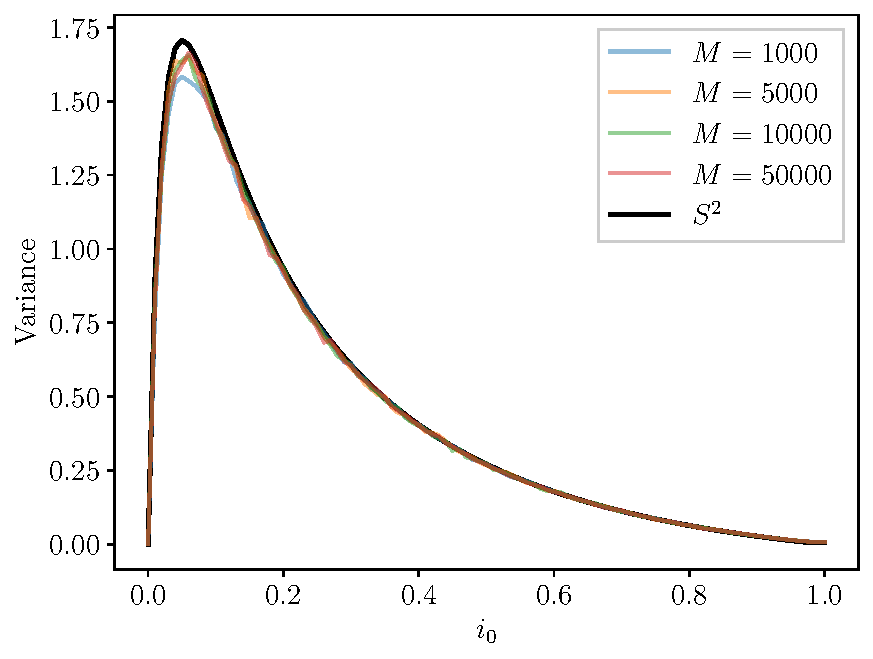
\includegraphics[width=\textwidth]{chp06_applications/figures/sir/sir_s2_1.0_1.0.pdf}
		% 			\caption{\(\beta = 2.0\), \(\gamma = 1\) (\(R_0 = 1\))}
		% 		\end{subfigure}
		\caption{The stochastic sensitivity value (in black) of the SIR diffusion limit \cref{eqn:sir_diff_limit} at time \(T = 5\), for varying initial condition \((1 - i_0, i_0)^{\T}\).
			The maximum projection of the sample covariance matrix (in various colours) for \(N = 10000\) stochastic simulations of the discrete population process over the same time interval is included.
			The corresponding initial condition is \(\left((1 - i_0)M, i_0 M\right)^{\T}\)}
		\label{fig:}
	\end{center}
\end{figure}






\subsection{Example 2: Ebola model with 6 compartments}\label{sec:epi_5d}
For our final example, we take a 6-compartment population process model that was used by \citet{LegrandEtAl_2007_UnderstandingDynamicsEbola} to analyse outbreaks of Ebola in the Democratic Republic of Congo in 1995 and in Uganda in 2000.


For a fixed population size, this model is 5-dimensional.

\begin{figure}
	\begin{center}
		\begin{tabular}{|c|c|c|c|}
			\hline
			Transition & \multicolumn{2}{c|}{Event}    & Rate \(\lambda_i\)                                                                                                     \\ \hline
			(1)        & Exposure                      & \(\left(S, E\right) \to \left(S-1, E+1\right)\)     & \(\left(\beta_I SI + \beta_H SH + \beta_F SF\right) / N\)        \\ \hline
			(2)        & Shedding                      & \(\left(E, I\right) \to \left(E - 1, I + 1\right)\) & \(\alpha E\)                                                     \\ \hline
			(3)        & Hospitalisation               & \(\left(I, H\right) \to \left(I - 1, H + 1\right)\) & \(\gamma_H \theta_1 I\)                                          \\ \hline
			(4)        & Hospital death without burial & \(\left(H, D\right) \to (H - 1, D + 1)\)            & \(\gamma_{dh}\delta_2 H\)                                        \\ \hline
			(5)        & Burial                        & \(\left(D\right) \to \left(D - 1\right)\)           & \(\gamma_f D\)                                                   \\ \hline
			(6)        & Death with burial             & \(\left(I\right) \to \left(I - 1\right)\)           & \(\gamma_i\left(1 - \theta_1\right)\left(1 - \delta_1\right) I\) \\ \hline
			(7)        & Death without burial          & \(\left(I, D\right) \to \left(I - 1, D + 1\right)\) & \(\delta_1 \left(1 - \theta_1\right) \gamma_d I\)                \\ \hline
			(8)        & Hospital death with burial    & \(\left(H\right) \to \left(H - 1\right)\)           & \(\gamma_{ih}\left(1 - \delta_2\right)H\)                        \\ \hline
		\end{tabular}

		\begin{tikzpicture}
			\node (S) [draw] {S};
			\node (E) [draw, right=of S] {E};
			\node (I) [draw, right=of E] {I};
			\node (H) [draw, right=of I] {H};
			\node (F) [draw, right=of H] {F};
			\node (R) [draw, right=of F] {R};
			\path[->,thick] (S) edge[above] node{(1)}  (E)
			(E) edge[above] node{(2)} (I)
			(I) edge[above] node{(3)} (H)
			(H) edge[above] node{(4)} (F)
			(F) edge[above] node{(5)} (R)
			(I) edge[bend right, below] node{(6)} (R)
			(I) edge[bend right, below] node{(7)} (F)
			(H) edge[bend left, above] node{(8)} (R);
		\end{tikzpicture}
		\caption{Transition probabilities of the Ebola model.}
		\label{fig:ebola_transition}
	\end{center}
\end{figure}


Let \(X_t^{(N)} = \left(S_t / N, I_t / N, E_t / N, H_t / N, D_t / N\right)^{\T}\) denote the proportion of individuals in each compartment at time \(t\).
The population process is also density dependent, with
\[
	f\!\left(\left(s, e, i, h, d\right), l\right) = \begin{cases}
		\beta_I s i + \beta_H sh + \beta_F sd,                        & \text{if } l = \left(-1, 1, 0, 0, 0\right), \\
		\alpha e,                                                     & \text{if } l = \left(0, -1, 1, 0, 0\right), \\
		\gamma_h \theta_1 i,                                          & \text{if } l = \left(0, 0, -1, 1, 0\right), \\
		\gamma_{dh}\delta_2 h,                                        & \text{if } l = \left(0, 0, 0, -1, 1\right), \\
		\gamma_f d,                                                   & \text{if } l = \left(0, 0, 0, 0, -1\right), \\
		\gamma_i\left(1 - \theta_1\right)\left(1 - \delta_1\right) i, & \text{if } l = \left(0,0,-1,0,0\right),     \\
		\delta_1\left(1 - \theta_1\right)\gamma_d i,                  & \text{if } l = \left(0,0,-1,0,1\right),     \\
		\gamma_{ih}\left(1 - \delta_2\right)h,                        & \text{if } l = \left(0,0,0,-1,0\right),     \\
		0,                                                            & \text{otherwise}.
	\end{cases}
\]
The deterministic differential equation is
\[
	\dod{X_t^{(\infty)}}{t} = \begin{bmatrix}
		-\beta_I X_t^{(\infty, 1)}X_t^{(\infty, 3)} - \beta_H X_t^{(\infty, 1)}X_t^{(\infty, 4)} - \beta_F X_t^{(\infty, 1)}X_t^{(\infty,5)}                                        \\
		\beta_I X_t^{(\infty, 1)}X_t^{(\infty, 3)} + \beta_H X_t^{(\infty, 1)}X_t^{(\infty, 4)} + \beta_F X_t^{(\infty, 1)}X_t^{(\infty,5)} - \alpha X_t^{(\infty, 2)}              \\
		\alpha X_t^{(\infty, 2)} - \left(\gamma_h + \gamma_i\left(1 - \theta_1\right)\left(1 - \delta_1\right) + \delta_1\left(1 - \theta_1\right)\gamma_d\right) X_t^{(\infty, 3)} \\
		\gamma_h\theta_1 X_t^{(\infty, 3)} - \gamma_{dh}\delta_2 X_t^{(\infty, 4)} - \gamma_{ih}\left(1 - \delta_2\right)X_t^{(\infty,4)}                                           \\
		\gamma_{dh}\delta_2 X_t^{(\infty, 4)} + \delta_1\left(1 - \theta_1\right)\gamma_d X_t^{(\infty, 3)} - \gamma_f X_t^{(\infty, 5)}
	\end{bmatrix}.
\]
The \(5\times 5\) diffusion matrix \(g\) satisfies

\begin{scriptaligned}
	\left[g\!\left(X_t^{(\infty)}\right)g\!\left(X_t^{(\infty)}\right)^{\T}\right]_{11} & =	\beta_I X_t^{(\infty, 1)} X_t^{(\infty, 2)} + \beta_H X_t^{(\infty, 1)} X_t^{(\infty, 4)} + \beta_F X_t^{(\infty, 1)} X_t^{(\infty, 5)} \\
	\left[g\!\left(X_t^{(\infty)}\right)g\!\left(X_t^{(\infty)}\right)^{\T}\right]_{12} = \left[g\!\left(X_t^{(\infty)}\right)g\!\left(X_t^{(\infty)}\right)^{\T}\right]_{21} & =  -\beta_I X_t^{(\infty, 1)} X_t^{(\infty, 2)} - \beta_H X_t^{(\infty, 1)} X_t^{(\infty, 4)} - \beta_F X_t^{(\infty, 1)} X_t^{(\infty, 5)} \\
	\left[g\!\left(X_t^{(\infty)}\right)g\!\left(X_t^{(\infty)}\right)^{\T}\right]_{22} & = \beta_I X_t^{(\infty, 1)} X_t^{(\infty, 2)} + \beta_H X_t^{(\infty, 1)} X_t^{(\infty, 4)} + \beta_F X_t^{(\infty, 1)} X_t^{(\infty, 5)} +  \alpha X_t^{(\infty, 2)} \\
	\left[g\!\left(X_t^{(\infty)}\right)g\!\left(X_t^{(\infty)}\right)^{\T}\right]_{23} = \left[g\!\left(X_t^{(\infty)}\right)g\!\left(X_t^{(\infty)}\right)^{\T}\right]_{32} & = -\alpha X_t^{(\infty, 2)} \\
	\left[g\!\left(X_t^{(\infty)}\right)g\!\left(X_t^{(\infty)}\right)^{\T}\right]_{33} & = \alpha X_t^{(\infty, 2)} + \left(\gamma_H \theta_1  + \gamma_i(	1 - \theta_1)(1 - \delta_1) + \delta_1(1 - \theta_1)\gamma_d\right)X_t^{(\infty, 1)} \\
	\left[g\!\left(X_t^{(\infty)}\right)g\!\left(X_t^{(\infty)}\right)^{\T}\right]_{34} = \left[g\!\left(X_t^{(\infty)}\right)g\!\left(X_t^{(\infty)}\right)^{\T}\right]_{43} & = - \gamma_H \theta_1 X_t^{(\infty, 1)}\\
	\left[g\!\left(X_t^{(\infty)}\right)g\!\left(X_t^{(\infty)}\right)^{\T}\right]_{35} = \left[g\!\left(X_t^{(\infty)}\right)g\!\left(X_t^{(\infty)}\right)^{\T}\right]_{53} & = - \delta_1(1 - \theta_1)\gamma_d X_t^{(\infty, 1)}\\
	\left[g\!\left(X_t^{(\infty)}\right)g\!\left(X_t^{(\infty)}\right)^{\T}\right]_{44} & = \gamma_H \theta_1 X_t^{(\infty, 1)} + \left(\gamma_{dh}\delta_2  + \gamma_{ih}(1 - \delta_2)\right)X_t^{(\infty, 4)} \\
	\left[g\!\left(X_t^{(\infty)}\right)g\!\left(X_t^{(\infty)}\right)^{\T}\right]_{45} = \left[g\!\left(X_t^{(\infty)}\right)g\!\left(X_t^{(\infty)}\right)^{\T}\right]_{54} & = -\gamma_{dh}\delta_2 X_t^{(\infty, 4)} \\
	\left[g\!\left(X_t^{(\infty)}\right)g\!\left(X_t^{(\infty)}\right)^{\T}\right]_{55} & = \delta_1(1 - \theta_1)\gamma_d X_t^{(\infty, 1)} + \gamma_{dh}\delta_2 X_t^{(\infty, 4)} + \gamma_f X_t^{(\infty, 5)}
\end{scriptaligned}
with all other entries zero.
There are many choices of \(g\) such that the product \(gg^{\T}\) has these entries, but to compute the Gaussian approximation with Mazzoni's method, we only need to evaluate \(g\!\left(X_t^{(\infty)}\right)g\!\left(X_t^{(\infty)}\right)\) and therefore no not need to make such a choice.






\DeclareSIUnit\week{week}
\begin{table}
	\begin{center}
		\begin{tabular}{|c|c|c|}
			\hline
			Parameter             & Value                       & Source                                                                            \\ \hline
			Population size \(N\) & 200000                                                                                                          \\
			Initial cases \(I_0\) & 3                                                                                                               \\
			\(\alpha\)            & \(1 / 7\) \unit{\per\day}                                                                                       \\
			\(\gamma_h\)          & \(1 / 9.6\) \unit{\per\day}                                                                                     \\
			\(\gamma_i\)          & \(1 / 10\) \unit{\per\day}                                                                                      \\
			\(\gamma_f\)          & \(1 / 2\) \unit{\per\day}                                                                                       \\
			\(\theta_1\)          & \(0.67\)                                                                                                        \\
			\(\delta_1\)          & \(0.8\)                                                                                                         \\
			\(\delta_2\)          & \(0.8\)                                                                                                         \\
			\(\beta_I\)           & \(0.588\) \unit{\per\week}  & \multirow{3}{*}{Estimated by \citet{LegrandEtAl_2007_UnderstandingDynamicsEbola}} \\
			\(\beta_H\)           & \(0.794\) \unit{\per\week}  &                                                                                   \\
			\(\beta_F\)           & \(7.653\) \unit{\per\week}  &                                                                                   \\
			\hline
		\end{tabular}
	\end{center}
	\caption{Parameter values for the Ebola model, estimated from the 1995 outbreak in the Democratic Republic of Congo.}
	\label{tab:ebola_param_vals}
\end{table}





\begin{figure}
	\begin{center}
		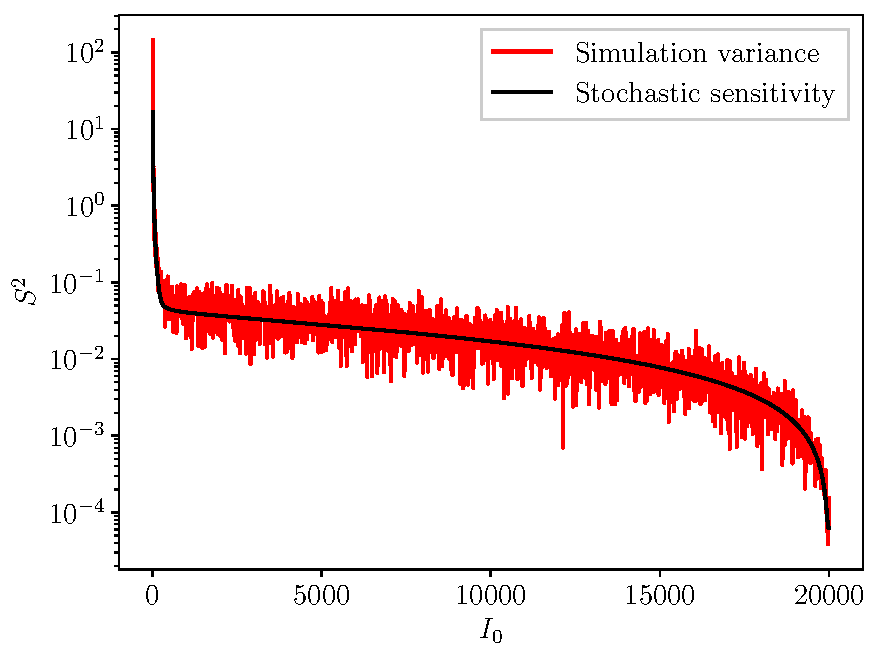
\includegraphics[width=\textwidth]{chp06_applications/figures/seihfr/seihfr_s2.pdf}
		\caption{}
		\label{fig:}
	\end{center}
\end{figure}
